\documentclass[a4paper,11pt,fleqn,oneside, openright]{memoir} % Brug openright hvis chapters skal starte p� h�jresider; openany, oneside

%%%% PACKAGES %%%%

% �� Overs�ttelse og tegns�tning �� %
\usepackage[utf8]{inputenc}					% G�r det muligt at bruge �, � og � i sine .tex-filer
\usepackage[danish]{babel}							% Dansk sporg, f.eks. tabel, figur og kapitel
\usepackage[T1]{fontenc}								% Hj�lper med orddeling ved �, � og �. S�tter fontene til at %v�re ps-fonte, i stedet for bmp	
\usepackage{latexsym}										% LaTeX symboler
\usepackage{xcolor,ragged2e,fix-cm}			% Justering af elementer
\usepackage{pdfpages}										% G�r det muligt at inkludere pdf-dokumenter med kommandoen \includepdf[pages={x-y}]{fil.pdf}	
\pretolerance=2500 											% G�r det muligt at justre afstanden med ord (h�jt tal, mindre orddeling og mere space mellem ord)
\usepackage{ulem}                       % Gennemstregning af ord med koden \sout{}
\usepackage{fixltx2e}										% Retter forskellige bugs i LaTeX-kernen
\usepackage{gensymb}					%Tilføjer \celsius og \degree notation	
\usepackage{lineno}						%Bruges til at tilføje linjetal
																	
% �� Figurer og tabeller � floats  �� %
\usepackage{flafter}										% S�rger for at dine floats ikke optr�der i teksten f�r de er sat ind.
\usepackage{multirow}                		% Fletning af r�kker
\usepackage{hhline}                   	% Dobbelte horisontale linier
\usepackage{multicol}         	        % Fletning af kolonner
\usepackage{colortbl} 									% Mulig�re farver i tabeller
%\usepackage{float}												% G�r det muligt at placere figurer hvor du vil.   \begin{figure}[!h] % Will not be floating.
\usepackage{wrapfig}										% Inds�ttelse af figurer omsv�bt af tekst. \begin{wrapfigure}{Placering}{St�rrelse}
\usepackage{graphicx} 									% Pakke til jpeg/png billeder
\pdfoptionpdfminorversion=6							% Muligg�r inkludering af pdf dokumenter, af version 1.6 og h�jere
	
% �� Matematiske formler og maskinkode ��
\usepackage{amsmath,amssymb,stmaryrd} 	% Bedre matematik og ekstra fonte
\usepackage{textcomp}                 	% Adgang til tekstsymboler
\usepackage{mathtools}									% Udvidelse af amsmath-pakken. 
\usepackage{eso-pic}										% Tilf�j billedekommandoer p� hver side
\usepackage{lipsum}											% Dummy text \lipsum[..]
\usepackage{rsphrase}										% Kemi-pakke til RS-s�tninger
\usepackage[version=3]{mhchem} 					% Kemi-pakke til lettere notation af formler

% �� Referencer, bibtex og url'er �� %
\usepackage{url}												% Til at s�tte urler op med. Virker sammen med hyperref
\usepackage[danish]{varioref}						% Giver flere bedre mulighed for at lave krydshenvisninger
\usepackage{natbib}											% Litteraturliste med forfatter-�r og nummerede referencer
\usepackage{xr}													% Referencer til eksternt dokument med \externaldocument{<NAVN>}

% �� Floats �� %
%\let\newfloat\relax 										% Memoir har allerede defineret denne, men det g�r float pakken ogs�
%\usepackage{float}

\usepackage[footnote,draft,danish,silent,nomargin]{fixme}		% Inds�t rettelser og lignende med \fixme{...} Med final i stedet for draft, udl�ses en error 																															for hver fixme, der ikke er slettet, n�r rapporten bygges.

%%%% CUSTOM SETTINGS %%%%

% �� Marginer �� %
\setlrmarginsandblock{3.5cm}{2.5cm}{*}	% \setlrmarginsandblock{Indbinding}{Kant}{Ratio}
\setulmarginsandblock{2.5cm}{3.0cm}{*}	% \setulmarginsandblock{Top}{Bund}{Ratio}
\checkandfixthelayout 									% Laver forskellige beregninger og s�tter de almindelige l�ngder op til brug ikke memoir pakker

%	�� Afsnitsformatering �� %
\setlength{\parindent}{0mm}           	% St�rrelse af indryk
\setlength{\parskip}{4mm}          			% Afstand mellem afsnit ved brug af double Enter
\linespread{1,1}												% Linie afstand

% �� Litteraturlisten �� %
\bibpunct[,]{[}{]}{;}{a}{,}{,} 					% Definerer de 6 parametre ved Harvard henvisning (bl.a. parantestype og seperatortegn)
%\bibliographystyle{bibtex/harvard}			% Udseende af litteraturlisten. Ligner dk-apali - mvh Klein

% �� Indholdsfortegnelse �� %
\setsecnumdepth{subsection}		 					% Dybden af nummerede overkrifter (part/chapter/section/subsection)
\maxsecnumdepth{subsection}							% �ndring af dokumentklassens gr�nse for nummereringsdybde
\settocdepth{section} 								% Dybden af indholdsfortegnelsen

% �� Visuelle referencer �� %
\usepackage[colorlinks=true]{hyperref}			 	% Giver mulighed for at ens referencer bliver til klikbare hyperlinks. .. [colorlinks]{..}
\hypersetup{pdfborder = 0}							% Fjerner ramme omkring links i fx indholsfotegnelsen og ved kildehenvisninger ��
\hypersetup{														%	Ops�tning af farvede hyperlinks
    colorlinks = true,
    linkcolor = black,
    anchorcolor = black,
    citecolor = black,
    urlcolor = black
}

\definecolor{gray}{gray}{0.80}					% Definerer farven gr�

% �� Ops�tning af figur- og tabeltekst �� %
 	\captionnamefont{
 		\small\bfseries\itshape}						% Ops�tning af tekstdelen ("Figur" eller "Tabel")
  \captiontitlefont{\small}							% Ops�tning af nummerering
  \captiondelim{. }											% Seperator mellem nummerering og figurtekst
  \hangcaption													%	Venstrejusterer flere-liniers figurtekst under hinanden
  \captionwidth{\linewidth}							% Bredden af figurteksten
	\setlength{\belowcaptionskip}{10pt}		% Afstand under figurteksten
		
% �� Navngivning �� %
\addto\captionsdanish{
	\renewcommand\appendixname{Appendiks}
	\renewcommand\contentsname{Indholdsfortegnelse}	
	\renewcommand\appendixpagename{Appendiks}
%	\renewcommand\cftchaptername{\chaptername~}				% Skriver "Kapitel" foran kapitlerne i indholdsfortegnelsen
	\renewcommand\cftappendixname{\appendixname~}			% Skriver "Appendiks" foran bilagene i indholdsfortegnelsen
	\renewcommand\appendixtocname{Appendiks}
}

% �� Kapiteludssende �� %
\definecolor{numbercolor}{gray}{0.7}			% Definerer en farve til brug til kapiteludseende
\newif\ifchapternonum

\makechapterstyle{jenor}{									% Definerer kapiteludseende -->
  \renewcommand\printchaptername{}
  \renewcommand\printchapternum{}
  \renewcommand\printchapternonum{\chapternonumtrue}
  \renewcommand\chaptitlefont{\fontfamily{pbk}\fontseries{db}\fontshape{n}\fontsize{25}{35}\selectfont\raggedleft}
  \renewcommand\chapnumfont{\fontfamily{pbk}\fontseries{m}\fontshape{n}\fontsize{1in}{0in}\selectfont\color{numbercolor}}
  \renewcommand\printchaptertitle[1]{%
    \noindent
    \ifchapternonum
    \begin{tabularx}{\textwidth}{X}
    {\let\\\newline\chaptitlefont ##1\par} 
    \end{tabularx}
    \par\vskip-2.5mm\hrule
    \else
    \begin{tabularx}{\textwidth}{Xl}
    {\parbox[b]{\linewidth}{\chaptitlefont ##1}} & \raisebox{-15pt}{\chapnumfont \thechapter}
    \end{tabularx}
    \par\vskip2mm\hrule
    \fi
  }
}																						% <--

\chapterstyle{jenor}												% Valg af kapiteludseende - dette kan udskiftes efter �nske

% �� Sidehoved �� %

%\makepagestyle{custom}																				% Definerer sidehoved og sidefod - kan modificeres efter �nske -->
%\makepsmarks{custom}{																						
%\def\chaptermark##1{\markboth{\itshape\thechapter. ##1}{}}		% Henter kapitlet den p�g�ldende side h�rer under med kommandoen \leftmark. \itshape g�r teksten kursiv
%\def\sectionmark##1{\markright{\thesection. ##1}{}}					% Henter afsnittet den p�g�ldende side h�rer under med kommandoen \rightmark
%}																														% Sidetallet skrives med kommandoen \thepage	
%\makeevenhead{custom}{Gruppe B130}{}{\leftmark}							% Definerer lige siders sidehoved efter modellen \makeevenhead{Navn}{Venstre}{Center}{H�jre}
%\makeoddhead{custom}{\rightmark}{}{Aalborg Universitet}			% Definerer ulige siders sidehoved efter modellen \makeoddhead{Navn}{Venstre}{Center}{H�jre}
%\makeevenfoot{custom}{\thepage}{}{}													% Definerer lige siders sidefod efter modellen \makeevenfoot{Navn}{Venstre}{Center}{H�jre}
%\makeoddfoot{custom}{}{}{\thepage}														% Definerer ulige siders sidefod efter modellen \makeoddfoot{Navn}{Venstre}{Center}{H�jre}		
%\makeheadrule{custom}{\textwidth}{0.5pt}											% Tilf�jer en streg under sidehovedets indhold
%\makefootrule{custom}{\textwidth}{0.5pt}{1mm}								% Tilf�jer en streg under sidefodens indhold

%\copypagestyle{nychapter}{custom}														% F�lgende linier s�rger for, at sidefoden bibeholdes p� kapitlets f�rste side
%\makeoddhead{nychapter}{}{}{}
%\makeevenhead{nychapter}{}{}{}
%\makeheadrule{nychapter}{\textwidth}{0pt}
%\aliaspagestyle{chapter}{nychapter}													% <--

\pagestyle{plain}																							% Valg af sidehoved og sidefod

% �� Fjerner den vertikale afstand mellem listeopstillinger og punktopstillinger �� %
\let\olditemize=\itemize							
\def\itemize{\olditemize\setlength{\itemsep}{-1ex}}
\let\oldenumerate=\enumerate						
\def\enumerate{\oldenumerate\setlength{\itemsep}{-1ex}}

%%%% CUSTOM COMMANDS %%%%

% �� Billede hack �� %
\newcommand{\figur}[4]{
		\begin{figure}[H] \centering
			\includegraphics[width=#1\textwidth]{billeder/#2}
			\caption{#3}\label{#4}
		\end{figure} 
}

% �� Specielle tegn �� %
\newcommand{\grader}{^{\circ}C}
\newcommand{\gr}{^{\circ}}
\newcommand{\g}{\cdot}

% �� Promille-hack (\promille) �� %
\newcommand{\promille}{%
  \relax\ifmmode\promillezeichen
        \else\leavevmode\(\mathsurround=0pt\promillezeichen\)\fi}
\newcommand{\promillezeichen}{%
  \kern-.05em%
  \raise.5ex\hbox{\the\scriptfont0 0}%
  \kern-.15em/\kern-.15em
  \lower.25ex\hbox{\the\scriptfont0 00}}

%%%% ORDDELING %%%%

\hyphenation{hvad hvem hvor}

%%%% Tabeler %%%%
\usepackage{threeparttable}
\usepackage[tableposition=top]{caption}

%%%% listings %%%%
\usepackage{listings}
\lstset{language=C}
\lstset{backgroundcolor=,rulecolor=}
\lstset{commentstyle=\textit}
\usepackage{lastpage}

\usepackage{marvosym}

%%%% top/tail %%%%

%\newcommand{\toptail}[1]{\fboxsep2mm\fbox{\begin{minipage}{145.3mm}#1\end{minipage}}}

\newcommand{\Ohm}{\ohm}
\newcommand{\my}{\mu}
\newcommand{\kilde}[1]{\fixme{Kilde: #1}}

 \usepackage[electronic]{ifsym}

\title{P3 Rapport}
\author{311}

\begin{document}
\thispagestyle{empty}
\begin{center}
\textsc{\huge Analog og digital elektronik\\}
\vspace{5 mm}

\textsc{\Large ...\\}
\vspace{25 mm}

\textsc{\textbf{\HUGE Effektforstærker\\}}
\vspace{20 mm}

\begin{flushright}
P3 Projekt \\
School of Information and Communication Technology \\
Elektronik \& IT Aalborg Universitet \\
Efteråret 2010 \\
\end{flushright}


\includegraphics[width=1.0\textwidth]{forside/forside.png}

\end{center}

%Blank side
\thispagestyle{empty}
\newpage
\mbox{}
\thispagestyle{empty}
\mbox{}
\newpage
\begin{multicols}{2}

\includegraphics[scale=0.35]{forside/aau.png}

\small{\textbf{Titel:\\}
HiFi-forstærker}

\scriptsize{\textbf{School of Information and Communication Technology\\ Elektronik \& IT\\}
Adresse: Fredrik Bajers Vej 7\\
Telefon: 99 40 86 00\\
URL: esn.aau.dk \\}
\end{multicols}
\begin{multicols}{2}

\small{
\textbf{Tema:\\}
Analog og digital elektronik

\textbf{Projektperiode:\\}
EIT3, efteråret 2010

\textbf{Projektgruppe:\\}
311

\textbf{Gruppemedlemmer:\\}
Benjamin Krebs\\
Frederik Juul\\
Jacob Hansen\\
Jesper Knudsen\\
Jonas Hansen\\

\textbf{Vejleder:\\}
Jan H. Mikkelsen

\textbf{Vikarierende vejleder:\\}
Ole Kiel Jensen

\textbf{Sidetal:\\}
\pageref{LastPage}

\textbf{Oplagstal:\\}
7

\textbf{Bilagsantal og art:\\}
1 bilags-CD

\textbf{Afsluttet den:\\}
21/12-2010
\\
\textbf{Synopsis:}
}

\fbox{\begin{minipage}{2.8in}
Der er i dette projekt arbejdet med design og fremstilling af en HiFi-forstærker. Målet med en HiFi-forstærker er at forstærke et lydsignal, med så stor præcision som muligt. Fra standarder er der opstillet en række krav som er valgt at overholde.

HiFi-forstærkeren i dette projekt består af fire moduler: Forforstærker, indgangsvælger, volumenkontrol og effektforstærker. Forforstærkerens funktion er at forstærke et mikrofonsignal til linieniveau, for at det kan sendes ind på niveau med et liniesignal. Dette gør at de to signaler kan behandles éns.
Indgangsvælgeren benyttes til at vælge imellem mikrofonsignalet eller stereosignalet: Intet signal, begge signaler eller de enkelte signaler hver for sig kan vælges. Indgangsvælgeren samler desuden signalerne, og skalérer det endelige signal, så outputtet derfra altid vil være på samme niveau.
Volumenkontrollen dæmper det samlede signals amplitude, til et af brugeren ønsket niveau, for at formindske den endelige volumen.
Effektforstærkeren forstærker signalet, hvilket sørger for at der kan afsættes den krævede effekt i højtaleren.
\end{minipage}}
\newline
\end{multicols}

\textit{\scriptsize{Rapportens indhold er frit tilgængeligt, men offentliggørelse (med kildeangivelse) må kun ske efter aftale med forfatterne.}}
\newpage
\begin{multicols}{2}

\includegraphics[scale=0.35]{forside/aau.png}

\small{\textbf{Title:\\}
HiFi-amplifier}

\scriptsize{\textbf{School of Information and Communication Technology\\ Electronics \& IT\\}
Adress: Fredrik Bajers Vej 7\\
Telephone: 99 40 86 00\\
URL: esn.aau.dk \\}
\end{multicols}
\begin{multicols}{2}

\small{\textbf{Theme:\\}
Analog and digital electronics

\textbf{Project Period:\\}
P3, fall 2010

\textbf{Project Group:\\}
311

\textbf{Group Members:\\}
Benjamin Krebs\\
Frederik Juul\\
Jacob Hansen\\
Jesper Knudsen\\
Jonas Hansen\\

\textbf{Supervisor:\\}
Jan H. Mikkelsen

\textbf{Number of pages:\\}
\pageref{LastPage}

\textbf{Printed Copies:\\}
8

\textbf{Appendix Media:\\}
1 appendix-CD

\textbf{Finished:\\}
21/12-2010
\\
\textbf{Synopsis:}}

\fbox{\begin{minipage}{2.8in}

...

...

...

...

...

...

...

...

...

...

...

...

...

...

...

...

...

...

...

...

...

...

...

...

...

...

...

...

...

...

...

\end{minipage}}
\newline
\end{multicols}
\textit{\scriptsize{The content of this paper is freely available, but publication (with references) is only allowed with permission from the author.}}

\newpage
%Blank side
\thispagestyle{empty}
\mbox{}
\newpage

%Læsevejledning
\section*{Læsevejledning}
I denne rapport benyttes forskellige former for notation. Disse er som følger:

\begin{itemize}
\item \textbf{Henvisninger til litteratur} er markeret med $"$[1]$"$ hvor nummeret svarer til et nummer i litteraturlisten. Disse henvisninger er, i den elektroniske version af rapporten, links, så de kan klikkes på. Henvisninger som er brugt til en enkelt information er markeret umiddelbart efter denne information og henvisninger brugt til et helt afsnit er markeret umiddelbart efter afsnittet.

\item \textbf{Henvisninger til figur eller afsnit} er markeret med $"$se figur/afsnit x.x.x$"$ hvor nummeret svarer til afsnitsnummeret i indholdsfortegnelsen eller figurnummeret under en figur. Disse henvisninger er, i den elektroniske version af rapporten, links.

\item \textbf{Binære tal} markeres med et undersænket b. F.eks. "10011$_b$" 

\item \textbf{Accepttestafsnit} sluttes alle med en tabel, der opsummerer de opstillede krav i forhold til deres status. Der vil ikke blive henvist til denne tabel, udover her. Et bestået krav er markeret med "\checkmark" mens et ikke bestået krav markeres med "$\mathcal{X}$".
\end{itemize}
%Ordliste
\section*{Ordliste}
\begin{itemize}
\item \textbf{AAU} - Aalborg Universitet
\item \textbf{EMC} - Electromagnetic compatibility
\item \textbf{THD} - Total Harmonic Distortion
\end{itemize}

\newpage
%Forord
\chapter*{Forord}
\label{forord}
Denne rapport dokumenterer et 3. semester projekt, udarbejdet i perioden fra 2. september 2010 til 21. december 2010. Projektet er udført af gruppe 311 på Elektronik og IT-ingeniør uddannelsen på Aalborg Universitet. Temaet for dette semester er $"$Analog og digital elektronik$"$ og gruppen valgte $"$High Fidelity (Hi-Fi) forstærker med digital styring$"$ som undertema. I løbet af semesteret modtager gruppen undervisning i form af PE- og SE-kurser, som bliver holdt af Institut for Elektroniske Systemer. Gruppen tilegner sig desuden viden gennem en fri studieaktivitet. Omtalte kurser er:

\begin{table}[h]
\centering
\begin{tabular}{c c}
\textbf{PE-kurser:} & \textbf{SE-kurser:} \\
Måleteknik & Quasistatiske elektriske og magnetiske felter \\
Analog elektronik & Beregningsteknik indenfor elektronikområdet 1 \\
Tilbagekoblingsteori 1 & Grundlæggende AC-kredsløbsteori \\
Basal digitalteknik & \\
\end{tabular}
\label{tab:kurser1}
\end{table}
\begin{table}[h]
\centering
\begin{tabular}{c}
\textbf{Fri studieaktivitet:} \\
PCB design og fabrikation \\
\end{tabular}
\label{tab:kurser2}
\end{table}
Gruppen har i løbet af projektet bestræbet sig på at opbygge mest muligt af løsningen analogt, fremfor digitalt. Der er i løbet af rapporten nævnt, når et element er udviklet specielt med dette for øje.\\\\
Gruppe 311 består af: \\\\\\\\\\
\begin{table}[h]
\centering
\begin{tabular}{c c c}
$\overline{~~~~~~Benjamin~Krebs~~~~~~}$ & $\overline{~~~~~~Frederik~Juul~~~~~~}$ & $\overline{~~~~~~Jacob~Hansen~~~~~~}$\\
\end{tabular}
\label{tab:gruppemedlemmer1}
\end{table} \\\\\\
\begin{table}[h]
\centering
\begin{tabular}{c c}
$\overline{~~~~~~Jesper~Knudsen~~~~~~}$ & $\overline{~~~~~~Jonas~Hansen~~~~~~}$\\
\end{tabular}
\label{tab:gruppemedlemmer2}
\end{table}

%Blank side
\thispagestyle{empty}
\mbox{}

\newpage
\tableofcontents*

%Linjetal
\setpagewiselinenumbers
\modulolinenumbers[5]
\linenumbers

%Indledning
\section{Indledning}
\begin{frame}{Indledning}

\end{frame}

\section{Systemopbygning}
For at kunne finde krav til dette projekts HiFi-forstærker er det nødvendigt at vælge hvilke blokke denne skal bestå af. I dette projekt er der ikke udelukkende valgt at designe en HiFi-forstærker i sin simpleste form, men også at tilføje funktionalitetsudvidende elementer. Systemets opbygning, med adskilte funktionelle blokke, er illustreret på figur \ref{fig:hififorstaerker_opbygning}. Dette afsnit vil argumentere og forklare den valgte opbygning. 


\begin{figure}[h]
\centering
\includegraphics[scale=0.6]{indledende_analyse/systemopbygning/forstaerker_opbygning.png}
\caption{Opbygning af dette projekts HiFi-forstærker}
\label{fig:hififorstaerker_opbygning}
\end{figure}


\subsection*{Input blokke}
Det er valgt at der skal kunne tilsluttes to typer lydkilder til HiFi-forstærkeren; en mikrofon og en kilde som afgiver et liniesignal. Kilder som afgiver et liniesignal er blandt andre computere, de fleste mobiltelefoner og medieafspillere, hvilket er grundlaget for netop at vælge denne type indgang. 
Grundlaget for at vælge en mikrofonindgang er udelukkende for at kunne anvende en indgangsvælger og for ikke at lave to ens linjeindgange. Desuden præsenterer en mikrofonindgang en ny blok: forforstærker.

HiFi-forstærkeren skal udstyres med et frontpanel hvorpå alle knapper til justeringsmulighederne skal placeres, således at de er tilgængelige for brugeren. Justeringsmulighederne, som skal være tilgængelige for brugeren er equalizerbånd, volumen og valg af indgang.

\subsection*{Analoge blokke}

Udgangsspændningen fra en mikrofon er langt lavere end linieniveau. Derfor benyttes en forforstærker til at forstærke mikrofonens lave signal op på niveau med liniesignalet, således at de er sammenlignelige i resten af systemet.

For at kunne vælge 

Forforstærker
Indgangsvælger
Volumenkontrol
Tonekontrol
Effektforstærker

\subsection*{Digital styring}
Digital styring


\subsection*{Output blokke}
Displays
Monoudgang
%\section{HiFi-forstærkerens generelle opbygning}

\begin{figure}[h]
\centering
\includegraphics[scale=.6]{indledende_analyse/generel_effektforstaerker/forstaerker_opbygning.png}
\caption{Opbygning af HiFi-forstærker}
\label{}
\end{figure}
%\chapter{Lydindgangstyper}
\label{indgange}
\textbf{Analog}
\begin{itemize}
\item{Linie}
\item{Mikrofon}
\item{Grammofon (RIAA)}
\item{Dolby Surround}
\end{itemize}

\textbf{Digital}
\begin{itemize}
\item{S/PDIF}
\item{Dolby Digital}
\end{itemize}


%Valg af løsning
\chapter{Valg af løsning}
\label{valgafloesning}
Formålet med dette kapitel er til slut at opstille en kravspecifikation for projektets HiFi-forstærker. Alle kravene i kravspecifikationen skal være målbare, så de kan testes ved projektets afslutning, og begrundede i det omfang dette er muligt. Før det er muligt at opstille en sådan kravspecifikation, er det nødvendigt at dokumentere hvilke overvejelser som danner grundlag for de forskellige dele af kravspecifikationen. Disse overvejelser er derfor beskrevet, inden de i afsnit \ref{kravspecifikation} samles til den endelige kravspecifikation for projektets HiFi-forstærker. 


\section{Standarder}
\label{standarder}
I dette afsnit bliver der taget udgangspunkt i gældende standarder fra International Electrotechnical Commitee (IEC) og Deutsches Institut f\"{u}r Normung (DIN). Målet med standarder er at opstille nogle normer for hvad produkter skal leve op til, hvilket gøres for at standardisere markedet sådan at produkter fra forskellige producenter kan arbejde sammen og ikke kun virker med produkter fra samme producent. Kravene opstillet i standarderne er ikke lovkrav, men derimod retningslinier. Det er dog i de færrestes interesse ikke at overholde standarderne.
\newline
\newline
I dette projekt er der valgt at arbejde med tre forskellige standarder. De tre standarder der arbejdes med er IEC581 Part 6, IEC61938 1 udgave og DIN 45500 normen.


\subsection*{IEC581 Part 6 - Amplifiers}
\label{IEC581}
Standarden IEC581 har titlen $"$High fidelity audio equipment and systems; Minimum performance requirements$"$ og er fra 1979. I dette projekt er det valgt kun at anvende del 6 af standarden da kun denne del har relevans for projektet. Del 6 af standarden opstiller generele minimumskrav til hvad en HiFi-forstærker skal overholde. \cite{IEC581-6}%\fixme{Kilde til IEC581-6}
\newline
\newline
Den første værdi der er taget fra standarden siger hvad minimumskrav der er for udgangseffekten.
\newline
\newline
\textbf{Udgangseffekt}
\begin{itemize}
\item Der skal minimum være et output på 10 W per kanal og det skal overholde kravet om forvrængning
\item Hvis forstærkeren har mere end én kanal skal alle kanaler kunne levere minimum 10 W samtidig.
\item Forstærkeren skal kunne levere det fastsatte output indenfor THD afvigelse i mindst 10 min., med alle kanaler tændt og en temperatur mellem 15 °C og 35 °C. Relativt til 1 kHz.
\end{itemize}

Den anden værdi der er taget fra standarden fastsætter et minimum for hvilket frekvensområde forstærkeren skal arbejde indenfor.
\newline 
\newline
\textbf{Frekvensområde}
\begin{itemize}
\item Frekvensområdet skal som minimum gå fra 40 Hz til 16 kHz
\item Der må være en tolerance på $\pm$ 1,5 dB for signaler der ikke er kommet igennem en equalizer. Relativt til 1 kHz
\item Der må være en tolerance på $\pm$ 2 dB for signaler der er kommet igennem en equalizer. Relativt til 1 kHz
\end{itemize}


\subsection*{IEC61938 1. udgave}
\label{IEC61938}
Standarden IEC61938 har titlen $"$Audio-, video- og audiovisuelle systemer - Indbyrdes forbindelser og matchende værdier - Foretrukne matchende analoge signalværdier$"$ og er fra 1997. Standarden der er brugt i rapporten er 1. udgave. Standarden opstiller generelle minimumskrav for hvad en HiFi-forstærker skal overholde. \cite{IEC61938}%\fixme{Kilde til IEC61938} 
\newline
\newline
Den første værdi fra standarden fremsætter hvad der skal overholdes for en linieindgang\fixme{Jesper: Skal nok lige skrives at der vælges en linie- og en mikrofonindgang før der kommer standarder for sjovt nok lige præcis de to typer}
\newline
\newline
\textbf{Liniesignaler}
\begin{itemize}
\item Indgangsimpedansen skal være større eller lig med 22 k\ohm
\item Signalspændingssvinget skal være mellem 0,2 V og 2 V
\item Udgangsimpedansen skal højst være 2,2 k\ohm
\end{itemize}
Anden krav fra standarden fremsætter hvad der skal overholdes for en mikrofonindgang
\newline 
\newline
\textbf{Mikrofonsignal}
\begin{itemize}
\item Indgangsimpedansen skal være større eller lig med 22 k\ohm
\item Outputspændingen skal være mellem 0,2 V og 2 V
\item Udgangsimpedansen skal højest være 2,2 k\ohm
\end{itemize}

\subsection*{DIN 45500 normen}
\label{DIN45500}
DIN 45500 normens fulde titel er Deutsches Institut f\"{u}r Normung 45500. Denne norm gælder for audioudstyr og er taget med fordi den opsætter minimumkrav til hvad en HiFi-forstærker skal overholde. Normen er fra 1973. \cite{DIN45500}%\fixme{Kilde til DIN45500}
\newline
\newline
Den første værdi fra normen beskriver hvor meget en HiFi-forstærker må forvrænge.
\newline
\newline
\textbf{Harmonisk forvrængning}
\begin{itemize}
\item Forforstærker eller effektforstærker må maksimalt forvrænge 0,7 \%
\item Forforstærker og effektforstærker må maksimalt forvrænge 1,0 \%
\item Dette skal være overholdt i en effektbåndbredde fra 40 Hz til 12,5 kHz
\end{itemize}
Den anden værdi fra normen beskriver krav til belastningsimpedansen.
\newline 
\newline
\textbf{Belastningsimpedans}
\begin{itemize}
\item For højtalere skal belastningsimpedansen være enten 4 \ohm~eller 8 \ohm
\item For hovedtelefoner skal belastningsimpendansen være enten 200 \ohm~eller 400 \ohm
\item Tolerance på 20 \%
\end{itemize}
\section{Klasser}
\label{klasser}
En HiFi-forstærkers udgangstrin kan designes på forskellige måder alt efter hvilken funktionalitet der ønskes. De forskellige designs er opdelt i klasser. Klasserne er bestemt ud fra en karakteristik og ikke ud fra en bestemt opkobling af kredsløbet. Karakteristika, som er vigtige at tage i betragtning for udgangstrinnet i en HiFi-forstærker er virkningsgrad, strømvinkel og forvrængning. Virkningsgrad er givet ved hvor stor en procentdel af den totale effekt leveret af forsyning, der bliver afsat i loaden, i dette tilfælde højtaleren.
I dette afsnit vil der blive gjort rede for klasse A, B og AB samt forklaret hvilke fordele og ulemper der er med dem. Redegørelsen vil tage udgangspunkt i ovenstående karakteristika samt demonstrere en mulig opbygning af trinnet.
Der vil, på baggrund af dette afsnit, blive valgt en endelig udgangstrinsklasse til dette projekts HiFi-forstærker hvilket vil blive, et krav i kravspecifikationen.

\subsection{Klasse A}

Et klasse A udgangstrin har en strømkarakteristik på udgangen, som vist på figur \ref{fig:klassea} med en sinustone, som indgangssignal. 

\begin{figure}[ht]
\begin{minipage}[b]{0.5\linewidth}
\centering
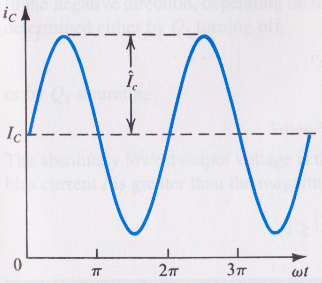
\includegraphics[scale=.35]{valg_af_loesning/klasser/klassea.png}
\caption{Klasse A $i_c$ karakteristik}
\label{fig:klassea}
\end{minipage}
\hspace{0.5cm}
\begin{minipage}[b]{0.5\linewidth}
\centering
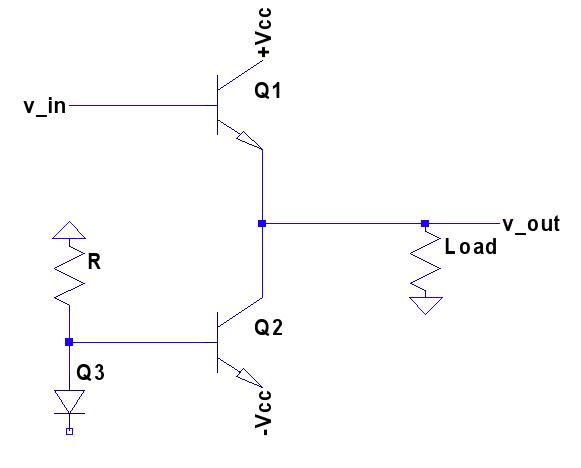
\includegraphics[scale=.35]{valg_af_loesning/klasser/classa.png}
\caption{Et eksempel på et klasse A forstærker kredsløb}
\label{fig:classa}
\end{minipage}
\end{figure}
\fixme{kilde: til sedra smith}


Et klasse A trin har en strømvinkel på udgangstransistoren på 360°. Dette viser sig nyttigt i det at indgangssignalet er repræsenteret på udgangen i sin komplette form, hvilket giver en lav forvrængning.
I et klasse A trin løber altid en konstant strøm gennem Q2, hvis kredsløbet på figur \ref{fig:classa} benyttes. Dette gør at den maksimale teoretiske virkningsgrad kun er 25\%. \fixme{kilde: til sedra smith}

Et klasse A udgangstrin kan opbygges af to NPN transistorer, Q1 og Q2, i en emitterfølgerkobling, som vist på figur \ref{fig:classa}. En konstant strøm løber gennem Q2, da $v_{BE2}$ er konstant. Inputsignalet kommer ind på Q1's base og styrer således strømmen der kan løbe gennem Q1 og loadmodstanden. 



\subsection{Klasse B}

Et klasse B udgangstrin har en strømkarakteristik på udgangen, som vist på figur \ref{fig:klasseb} med en sinustone, som indgangssignal. 

\begin{figure}[ht]
\begin{minipage}[b]{0.5\linewidth}
\centering
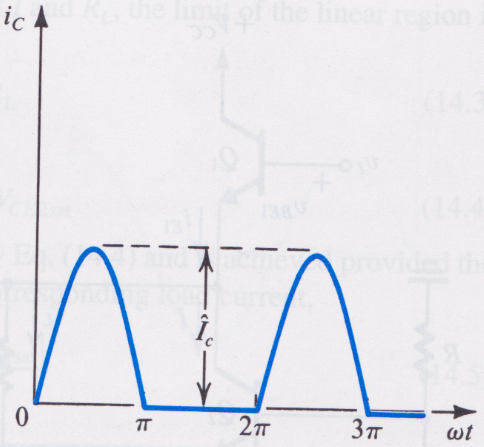
\includegraphics[scale=.35]{valg_af_loesning/klasser/klasseb.png}
\caption{Klasse B $i_c$ karakteristik}
\label{fig:klasseb}
\end{minipage}
\hspace{0.5cm}
\begin{minipage}[b]{0.5\linewidth}
\centering
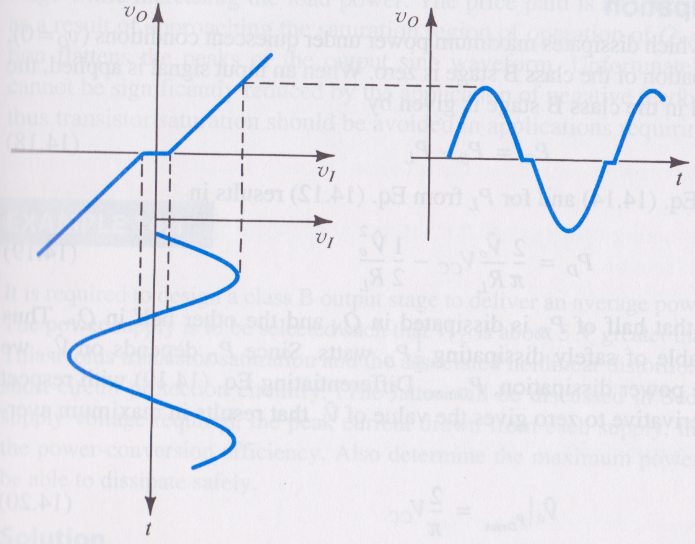
\includegraphics[scale=.25]{valg_af_loesning/klasser/klassebproblem.png}
\caption{Klasse B trin med crossoverdistortion}
\label{fig:classbproblem}
\end{minipage}
\end{figure}
\fixme{kilde: til sedra smith}
Et klasse B trin overfører kun en halv periode af indgangssignalet til udgangen, altså er strømvinklen 180°. For at kunne gengive et udgangssignal similært til indgangssignalet er det derfor nødvendigt at sammensætte to klasse B trin således at det ene tager sig af den positive halvperiode og den anden den negative. Dette giver anledning til et fænomen kaldet crossoverdistortion. Dette fænomen optræder i dette tilfælde i overgangen fra den positive halvperiode til den negative og skyldes diodekarakteristikken i transistorernes base-emitter. Crossoverdistortion for et klasse B trin er illustreret på figur \ref{fig:classbproblem}.
Et klasse B trin har en maksimal nyttevirkning på 78,5 \%.\fixme{kilde: til sedra smith}

I eksemplet er klasse B trinnet opbygget af to transistorer, en NPN (Q1) og en PNP (Q2), som vist på figur \ref{fig:classb}. Når input spændingen overstiger ca. 0,6 V vil Q1 begynde at lede strøm til loadmodstanden mens Q2 er lukket. Kommer input spændingen under -0,6 V vil Q2 lede, men da Q2 er en PNP vil den trække strøm mod -Vcc hvormed der trækkes strøm fra loadmodstanden. Når Q2 leder er Q1 lukket. 

\begin{figure}[h]
\centering
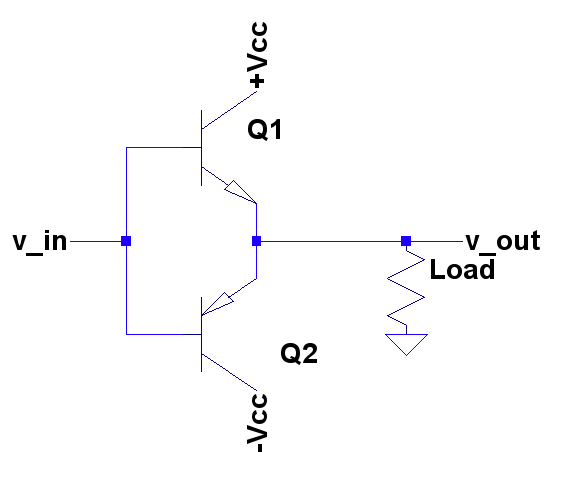
\includegraphics[scale=.35]{valg_af_loesning/klasser/classb.png}
\caption{Klasse B forstærker kredsløb}
\label{fig:classb}
\end{figure}

\subsection{Klasse AB}

Et klasse AB udgangstrin har en strømkarakteristik på udgangen, som vist på figur \ref{fig:klasseab} med en sinustone, som indgangssignal. 

\begin{figure}[ht]
\begin{minipage}[b]{0.5\linewidth}
\centering
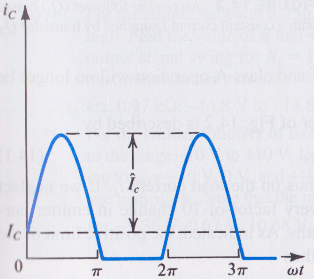
\includegraphics[scale=.35]{valg_af_loesning/klasser/klasseab.png}
\caption{Klasse AB $i_c$ karakteristik}
\label{fig:klasseab}
\end{minipage}
\hspace{0.5cm}
\begin{minipage}[b]{0.5\linewidth}
\centering
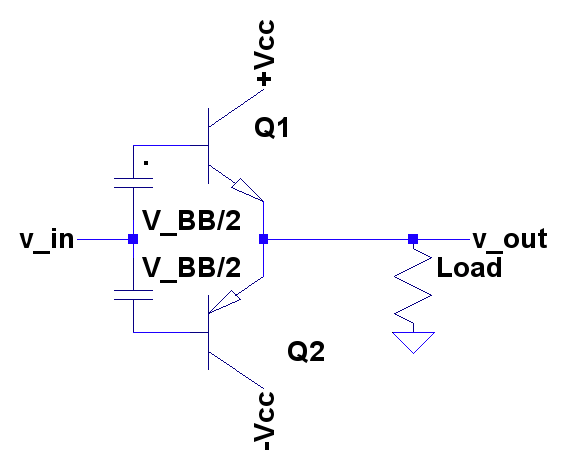
\includegraphics[scale=.35]{valg_af_loesning/klasser/classab.png}
\caption{Klasse AB forstærker kredsløb}
\label{fig:classab}
\end{minipage}
\end{figure}
\fixme{kilde: til sedra smith}


Dette trin har en strømvinkel på mellem 180 ° og 360 °. Dette bevirker at, hvis man bruger samme teknik, som ved et klasse B trin til at få en hel sinusperiode på udgangen, vil de to signaler overlappe i overgangsperioden. Dette medvirker til at crossoverdistortion, som forklaret for klasse B trinnet, elemineres. Dermed bliver forvrængningen for et klasse AB mindre end for et klasse B.
Et klasse AB trin har en nyttevirkning som ligger mellem den for et klasse A og et klasse B. \fixme{kilde: Jan ???}

Der tages i eksemplet på et klasse AB trin på figur \ref{fig:classab} udgangspunkt i klasse B trinnet på figur \ref{fig:classb}, med den forskel at potentialet på Q1 og Q2's base er hævet til saturationspændingen når signalspændningen er 0 V. Det er denne forskel, som eleminerer crossoverdistortion.

Et klasse AB udgangstrin har ikke et klasse A's lave nyttevirkning eller et klasse B's crossoverdistortion og er på baggrund af dette blevet valgt, som det udgangstrin der vil blive arbejdet videre på.
\section{Indgangsvælger}
\begin{frame}{Indgangsvælger - Krav}
\scriptsize{
\begin{table}[h]
\centering
\begin{tabular}{l|r}
\hline\hline
Område & Krav \\
\hline\hline
Antal trin i & 4 \\
indgangsvælgeren & \\[4pt]
Indgangsimpedans & \> 22 k\ohm \\[4pt]
Frekvensgang & \< 0,375 dB ved 20 Hz - 20 kHz, ref. 1 kHz \\
& \< 0,75 dB fra 20 Hz til 63 Hz \\
& \< 0,75 dB fra 12,5 kHz til 20 kHz \\[4pt]
Dæmpning af slukket & \> 50 dB ved 1 kHz \\
indgangssignal & \\
\hline\hline
\end{tabular}
\label{tab:krav_indgangsvaelger}
\end{table}
}
\end{frame}

\begin{frame}{Indgangsvælger - Opbygning}

\begin{figure}[h]
\centering
\includegraphics[width=\textwidth]{../rapport/teknisk/indgangsvaelger/signal-taend-sluk.png}
\label{fig:indgangsvaelger-overordnet}
\end{figure}
\end{frame}

\begin{frame}{Indgangsvælger - Styring}

\begin{figure}[h]
\centering
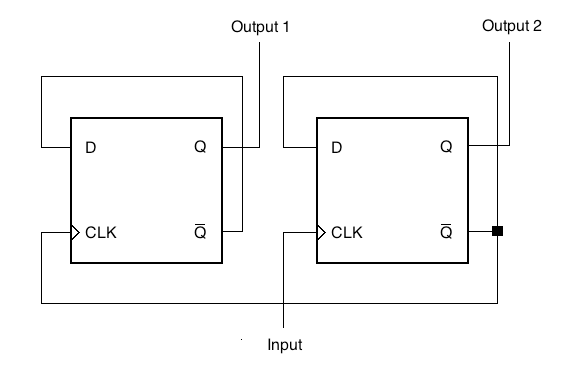
\includegraphics[scale=0.4]{../rapport/teknisk/indgangsvaelger/flipflop.png}
\label{fig:indgangsvaelger-flipflop}
\end{figure}
\end{frame}

\begin{frame}{Indgangsvælger - Simulering}
\begin{figure}[h]
\centering
\includegraphics[width=\textwidth]{../rapport/teknisk/indgangsvaelger/simulering/frekvenskarakteristik.png}
\label{indgangsvaelger_frekvenskarakteristik}
\end{figure}
\end{frame}

\begin{frame}{Indgangsvælger - Måling}
\begin{figure}[h]
\centering
\includegraphics[width=\textwidth]{../rapport/maalerapporter/indgangsvaelger/Indgangsvlger-mic-200mv-frek.png}
\label{fig:indacc:frek200mv}
\end{figure}
\end{frame}

\begin{frame}{Indgangsvælger - Måling}
\begin{figure}[h]
\centering
\includegraphics[width=\textwidth]{../rapport/maalerapporter/indgangsvaelger/Indgangsvlger-mic-2v-thd.png}
\label{fig:accind:thd2v}
\end{figure}
\end{frame}


\begin{frame}{Indgangsvælger - Oversigt}
\scriptsize{
\begin{table}[h]
\centering
\begin{tabular}{l|r|r}
\hline\hline
Område & Krav & Status \\
\hline\hline
Antal trin i & 4 & \checkmark \\
indgangsvælgeren & \\[4pt]
Indgangsimpedans & \> 22 k\ohm & \checkmark \\[4pt]
Frekvensgang & \< 0,375 dB ved 20 Hz - 20 kHz, ref. 1 kHz & \checkmark \\
& \< 0,75 dB fra 20 Hz til 63 Hz & \checkmark\\
& \< 0,75 dB fra 12,5 kHz til 20 kHz & \checkmark\\[4pt]
Dæmpning af slukket & \> 50 dB ved 1 kHz & \checkmark \\
indgangssignal & \\
\hline\hline
\end{tabular}
\label{tab:krav_indgangsvaelger}
\end{table}
}
\end{frame}
\section{Volumenkontrol}
\label{valg_volumenkontrol}
Kravet til styringen af volumenkontrol er sat til at dette skal foregå digitalt. Begrundelsen herfor ligger i projektets undertema, $"$High Fidelity (Hi-Fi) forstærker med digital styring$"$, og begrundes derfor ikke yderligere. Til bestemmelse af den maksimale dæmpning volumenkontrollen skal være i stand til, bruges samme krav som for slukkede signaler, altså 50 dB, som bestemt i afsnit \ref{standarder}. Volumenkontrollen skal derfor kunne dæmpe fra  0 dB til 50 dB. Desuden vælges størrelsen af hvert niveau til 1 dB, da dette er den mindste forskel et menneske kan opfatte i lydniveau \cite{lidt_om_lyd}. Dette sætter ydermere krav til at displayet, som opbygges af 7-segmenter, skal bestå af to 7-segmenter.\\
Volumen skal kunne justeres via trykknapper på HiFi-forstærkerens frontpanel, hvor det også skal være muligt at aflæse det øjeblikkelige volumenniveau.  

\section{Equalizer}
\label{equalizer}
Det menneskellige øre kan opfatte frekvenser fra ca. 20-20k Hz\fixme{kilde: http://www.hoerelse.info/page.dsp?page=414}. Dette sætter en naturligt bredde for frekvensbåndet, forstærkeren skal kunne operere indenfor. Udover at en given elektrisk komponent ikke vil være ens over hele frekvensbåndet, vil det akustiske miljø samt højtalerne også have indflydelse på den endelige oplevelse.  Derfor kan det være nødvendigt at regulere på de forskellige frekvenser, for at opnå den ønskede lyd. En equalizer benyttes til at dæmpe de forskellige frekvensbånd, i forhold til hinanden. En equalizer i en forstærker vil ofte være bredspektret og blive benyttet til at korrigere mere generelle ændringer i lyden. Hvis brugeren ønsker mere specifikke indstillinger, vil en dedikeret equalizer ofte benyttes. Da frekvensbåndet det menneskelige øre kan høre består af præcis 3 dekader, inddeles frekvensbåndene i equalizeren efter disse:
%Udtrykket equalizer stammer fra den originale hensigt med opfindelsen; at få det optagede til at lyde som den originale kilde. Dette gøres bl.a. for at kompensere for unøjagtigheder i optagelsesudstyr. Ved at dæmpe og forstærke individuelle frekvensbånd, er det muligt at få præcis den lyd brugeren kunne tænke sig. 
%En equalizer i en forstærker vil ofte være bredspektret og blive benyttet til at kompensere for det akustiske miljø brugeren befinder sig i, samt unøjagtigheder som følge af de benyttede komponenter. Hvis man har brug for mere specifikke indstillinger vil benyttet en dedikeret equalizer. Derfor har projektgruppen valgt at have 3 frekvensbånd\fixme{kilde: pdf dokument.}.

\begin{itemize}
\item Low: 20 - 200 Hz
\item Mid: 200 - 2000 Hz
\item High: 2000 - 20000 Hz
\end{itemize}

%Frekvensbåndene strækker sig fra 20 Hz til 20 kHz, da dette er det maksimale frekvensbånd det menneskelige øre kan opfatte\fixme{kilde: http://www.hoerelse.info/page.dsp?page=414}. Da dette frekvensbånd består af præcis 3 dekader, har projektgruppen valgt at inddele equalizerens frekvensbånd i disse.
%Hvor mange indstillingmuligheder der er på en equalizer, afhænger af antal af frekvensbånd, som kan indstilles uafhængigt af hinanden. Der opstilles derfor en række frekvensbånd, som et mål for projektet:
%Idéen med en equalizer er at kunne justere på styrken af de forskellige frekvenser i et signal, uafhængigt af hinanden. Dette benyttes til at få præcis den lyd, som brugeren ønsker. Eksempelvis kunne en bruger vælge at skrue op for de lave frekvenser, for at gøre bassen i et signal mere dominerende. I praksis er det dog en kombination af at forstærke nogle frekvensbånd, og dæmpe andre, på tværs af hele det hørbare område, for at skabe nøjagtigt den lyd der ønskes.\fixme{Skriv om} Dette er en hel videnskab i sig selv, men for at gøre mulighederne for dette så store som muligt, er det smart\fixme{andet ord?} at have et bredt udvalg af justerbare bånd. Dette gøres, analogt, ved hjælp af forskellige båndpas filtre.

\subsection{Visualizer}
\label{visualizer}
Visualizeren benyttes til at illustrere styrken af de signalerne i de forskellige frekvensbånd. I teorien kan en analog visualizer have uendeligt stor opløsning. I dette projekt vil det dog ikke give mening, ud fra et læringsmæssigt standpunkt at lave for stor opløsning, da dette bare er gentagelse af de samme basale elementer. Derimod vil en for lav opløsning heller ikke kunne bruges til noget. Derfor er en opløsning på seks dioder pr. frekvensbånd valgt. Dette giver desuden mulighed for at vise signalstyrken med farver: 2 grønne, efterfulgt af 2 gule, efterfulgt af 2 røde dioder.
%En visualizer giver et visuelt udtryk for, hvordan equalizeren er indstillet. Den angiver lydniveauet for hvert frekvensbånd, equalizeren dækker over. Dette giver bl.a. brugeren mulighed for at se hvilke frekvenser, der vil være optimale at justere på, for at få det ønskede output.
Vi startede ud med at beslutte os for, at måden vi skulle dæmpe signalet på, var at trække det til stel, før det blev summeret i summationsforstærkeren. Dette gave os at vi skulle have R3 og R4, for at kunne dæmpe signalet, uden at trække det endelige output til stel. Outputtet fra en gate er 5V, hvilket giver os V2. Der skal desuden løbe en basis strøm I_B, hvilket giver os modstanden R5. C1 er der for kun at få signalet over i indgangsvælger trinet. Vi fandt dog rimeligt hurtigt ud af at et spændingsving omkring 0V ville give prolemer med strøm løbende fra emitteren til collectoren i Q1, når signalet trækkes under 0V. Derfor blev vi enige om at lave et DC offset, hvilket vi gjorde med R1 og R2 samt V1. R1 og R2 er valgt til 100k hver, hvilket giver en spændingsdeling på 1:2 imellem dem, hvilket ved 15V giver et DC offset på 7.5V. R3 og R4 er valgt efter at have en indgangsimpedans over 22, både når indgangen er tændt og slukket. For at regne på dette AC mæssigt, kortsluttes kondensatorerne, hvilket betyder at R1 og R2 begge går til stel. Derfor sidder de i parallel, sammen med Re, som består af R3 og R4 i serie. Ved et slukket signal er der ideelt stel mellem R3 og R4, derfor er R4 ligegyldig her. For at regne R3 opstilles der en parallelkoblingsformel:
\begin{equation}
\frac{1}{\frac{1}{100}+\frac{1}{100}+\frac{1}{R}}=22
R=39.29
\end{equation}
Dette giver altså en R på ca. 40k, når signalet skal slukkes, hvilket altså vil sige R3. Når signalet så er tændt igen, er indgangsimpedansen højere, da R3 og R4 skal adderes. Vi har valgt en R4 på ca 7k, hvilket giver en total indgangsimpedans på:
\begin{equation}
\frac{1}{\frac{1}{100}+\frac{1}{100}+\frac{1}{40.2+7.32}}=24.36
\end{equation}
\section{Kortslutningssikring}
\label{valg_kortslutningssikring}
Der er opstillet krav om en kortslutningssikring for at sikre mod skader ved eventuelle overbelastninger på udgangen af HiFi-forstærkeren. Afsættes der $20~W$ i højtaleren, kan peakstrømmen bestemmes ved beregningen vist i formel (\ref{equ:ipeak}).

\begin{equation}
\label{equ:ipeak}
I_{\mathrm{peak}} = \sqrt{2 \cdot \frac{p_{\mathrm{RMS}}}{R}} = \sqrt{2 \cdot \frac{\mathrm{20~W}}{8~\ohm}}  = \mathrm{2,24~A}
\end{equation}

Denne peakstrøm fremkommer ved peakspændingen fundet i udregningen i formel (\ref{equ:vpeak}).

\begin{equation}
\label{equ:vpeak}
V_{\mathrm{peak}} = I_{\mathrm{peak}} \cdot R_{\mathrm{load}} = \mathrm{2,24~A \cdot 8~\ohm = 17,9~V}
\end{equation}

Ideelt vil en spændingsforsyning på 18 V altså være tilstrækkelig, dog er der rent praktisk behov for en større. Argumentationen herfor findes i afsnit \fixme{ref til udregninger ved effektforstærker}, hvor den ydermere bestemmes.
\section{Udgangseffekt}
\label{valg_udgangseffekt}
Fastsættelsen af udgangseffektens størrelse er bestemt af to faktorer. Den maksimale effekt der er mulig er bestemt af sikkerhedsreglerne i elektroniklaboratoriet på Aalborg Universitet. I disse regler angives den maksimale DC spænding der må arbejdes med til 60 V \cite{elregler-b1101}. 
Til projektets forstærker deles denne spænding til en forsyning som maksimalt kan være $\pm$ 30 V. Under udregningen af den maksimale effekt bruges RMS-værdien af den spænding. Desuden anvendes den, i afsnit \ref{standarder} valgte, belastningsmodstand på 8~\ohm. Dermed bliver den øvre grænse som vist i udregningen i formel (\ref{equ:maks_effekt}).

\begin{equation}
\label{equ:maks_effekt}
P_{\mathrm{max}} = \frac{(V_{\mathrm{RMS}})^2}{R_{\mathrm{load}}}= \frac{(\frac{\hat{V}}{\sqrt{2}})^2}{R_{\mathrm{load}}} = \frac{(\frac{\mathrm{30~V}}{\sqrt{2}})^2}{8~\ohm} = \mathrm{56,25~W}
\end{equation}

Den nedre grænse for udgangseffekten er defineret af standarden IEC581, i hvilken det er bestemt at udgangseffekten som minimum skal være 10 W, hvis der er tale om en monoudgang, før forstærkeren må kaldes en HiFi-forstærker, se afsnit \ref{standarder}. Kravet for udgangseffekten vælges til 20 W for dette projekts HiFi-forstærker.

\section{Udgangssignaltype}
\label{valg_udgangssignaltype}
Valget står for udgangssignaltypen mellem stereo og mono. Da stereo i princippet blot er et lydsignal med to kanaler i modsætning til mono, som er én kanal, vil fremstillingen af en stereoudgang på forstærkeren ikke umiddelbart være mere lærerig end fremstillingen af en monoudgang, den vil blot kræve mere tid. Af den årsag vælges udgangssignaltypen til mono.
\section{Total Harmonic Distortion}
\label{thd}
Total Harmonic Distortion, total harmonisk forvrængning - forkortet THD - er et udtryk for hvor meget forvrængning der er i et signal, fra kilden til output.  Hele kæden er med til at øge THD, da det er et biprodukt af, at komponenter ikke er lineære og derfor vil tilføje forvrængning til signalet. Jo højere THD, jo kraftigere overtoner, kendt på engelsk som harmonics\fixme{evt. i fodnote eller ordforklaring i stedet?}, vil der blive produceret, hvilket vil ændre det originale signal. Overtoner er frekvenser, som har et heltalsforhold\fixme{er det et ord?} til den originale frekvens; eksempelvis vil overtoner til 500Hz være 1000Hz, den dobbelte frekvens, og 1500Hz, tre gange frekvensen.\fixme{Skriv om med ligning} Disse overtoner bliver lagt til det originale signal; dette svarer til at det originale signal, er en slags AC-offset til de mindre kraftige overtoner, som set i figur \fixme{figur}. Det er derfor vigtigt at få så lav forvrængning som muligt, da hvert enkelt led i kæden, bidrager med sin egen. Så længe HiFi-forstærkerens totale forvrængning er under 1\% anses den dog som værende underordnet, da det ikke er muligt at detektere med det menneskelige øre.\fixme{kilde eller lav en ref til standarder}

\begin{figure}[h]
\centering
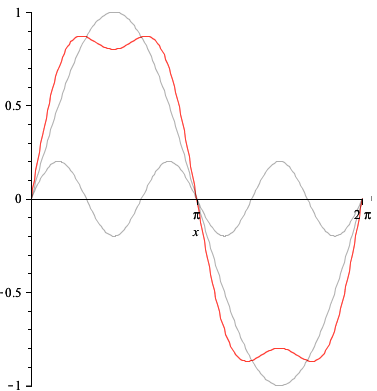
\includegraphics[scale=.4]{indledende_analyse/thd/thdsamlet.png}
\caption{Et eksempel på harmonisk forvrængning. Det originale signal virker som et AC-offset for den mindre kraftige, tredje harmoniske overtone.}
\label{fig:harmonic_distortion}
\end{figure}

\chapter{Kravspecifikation}
\label{kravspec}
Formålet med dette kapitel er til slut at opstille en kravspecifikation for projektets HiFi-forstærker. Alle kravene i kravspecifikationen skal være målbare, så de kan testes ved projektets afslutning, og begrundede i det omfang dette er muligt. Før det er muligt at opstille en sådan kravspecifikation, er det nødvendigt at dokumentere hvilke overvejelser som danner grundlag for de forskellige dele af kravspecifikationen. Der er i kapitel \ref{kap:indledende_analyse} ført dokumentation for en række af disse overvejelser. De resterende overvejelser er dokumenteret i de næste syv afsnit. I afsnit \ref{krav_krav} er produktet af alle disse overvejelser samlet i den endelige kravspecifikation for projektets HiFi-forstærker. 

\section{Indgangsvælger}
\label{krav_indgangsvaelger}
I forbindelse med indgangsvælgeren er overvejelserne gået på, hvorvidt denne skal lave en trinvis eller flydende overgang mellem indgangssignalerne. Da en flydende overgang i princippet er simultan volumenkontrol af indgangene, adskiller den form for indgangsvælger sig ikke i samme grad fra en egentlig volumenkontrol, som det er tilfældet med en trinvis indgangsvælger. Eftersom der er opstillet krav om en volumenkontrol til forstærkeren sættes kravet om indgangsvælgerens art til trinvis. \\
Som det fremgår i afsnit \ref{standarder} skal HiFi-forstærkeren have to indgange, hvilket danner grundlag for at kravet til antallet af trin i indgangsvælgeren sættes til tre. De tre trin er vist i tabel \ref{tab:indgangsvaelgertrin}.\fixme{Jesper: Har ikke lavet det med isolation, da jeg vil vente og se hvad Jacob skriver om det - ¿ Mener jeg hørte han fandt noget med det til standarder ?}

\begin{table}[h]
\centering
\begin{tabular}{c|c|c}
\hline\hline
Trin & Indgang 1 & Indgang 2 \\
\hline\hline
1 & On & Off \\
2 & Off & On \\
3 & On & On \\
\hline\hline
\end{tabular}
\caption{Indgangsvælgertrin}
\label{tab:indgangsvaelgertrin}
\end{table}

Valget mellem de tre trin skal kunne tages af brugeren på HiFi-forstærkerens frontpanel. Det skal desuden være tydeligt hvilket trin indgangsvælgeren er sat på.

\section{Indgangsimpedans}
\label{krav_indgangsimpedans}
Indgangsimpedansen er at opfatte som en impedans der, ud fra en almindelig spændingsdeling, reducerer indgangssignalet. Man er, med den begrundelse, interesseret i en stor indgangsimpedans. Den mindste tilladte størrelse af indgangsimpedansen for en HiFi-forstærker er i standard IEC61938-1 bestemt til 22 k\ohm~ for liniesignalsindgange, se afsnit \ref{standarder}. Da størrelsen af udgangsimpedansen samtidig er bestemt til maksimalt 2,2 k\ohm~ for en liniesignalsudgang, kan betydningen af indgangsimpedansens størrelse regnes som vist i udregningen i formel (\ref{equ:indgangsimpedans22}). 

\begin{equation}
\label{equ:indgangsimpedans22}
\frac{22~k\ohm}{22~k\ohm + 2,2~k\ohm} = 0,91
\end{equation}

Det ses af udregningen i formel (\ref{equ:indgangsimpedans22}), at en indgangsimpedans af størrelsen 22 k\ohm~ vil medføre et indgangssignal på 91 \% af det oprindelige signal. Med en større indgangsimpedans vil en større del af det oprindelige signal blive indgangssignalet. 

\begin{equation}
\label{equ:indgangsimpedans475}
\frac{47,5~k\ohm}{47,5~k\ohm + 2,2~k\ohm} = 0,96
\end{equation}

Udregningen i formel (\ref{equ:indgangsimpedans475}) viser at med en indgangsimpedans af størrelsen 47,5 k\ohm~ bliver indgangssignalet 96 \% af det oprindelige signal.

\section{Volumenkontrol}
\label{krav_volumenkontrol}
Kravet til styringen af volumenkontrol er sat til at dette skal foregå digitalt. Begrundelsen herfor ligger i det samtidige krav om volumenkontrol via fjernbetjening, læs mere herom i afsnit \ref{krav_fjernbetjening}. Volumen skal desuden kunne justeres via HiFi-forstærkerens frontpanel, hvor det også skal være muligt at aflæse det øjeblikkelige volumenniveau.  

\section{Udgangssignaltype}
\label{krav_udgangssignaltype}
Valget står for udgangssignaltypen mellem stereo og mono. Da stereo i princippet blot er et lydsignal med to kanaler i modsætning til mono, som er én kanal, vil fremstillingen af en stereoudgang på forstærkeren ikke umiddelbart være mere lærerig end fremstillingen af en monoudgang, den vil blot kræve mere tid.

\section{Udgangseffekt}
\label{krav_udgangseffekt}
Fastsættelsen af udgangseffektens størrelse er bestemt af to faktorer. Den maksimale effekt der er mulig er bestemt af sikkerhedsreglerne i elektronikværkstedet på Aalborg Universitet. I disse regler angives den maksimale DC spænding der må arbejdes med til 60 V \cite{elregler-b1101}. 
Til projektets forstærker deles denne spænding til en $\pm$30 V forsyning. Under udregningen af den maksimale effekt bruges RMS-værdien (Root Mean Square) af den spænding. Dermed bliver den øvre grænse som vist i udregningen i formel (\ref{equ:maks_effekt}).

\begin{equation}
\label{equ:maks_effekt}
P_{maks} = \frac{(V_{RMS})^2}{R}= \frac{(\frac{\hat{V}}{\sqrt{2}})^2}{R} = \frac{(\frac{30~V}{\sqrt{2}})^2}{8\ohm} = 56,25~W
\end{equation}

Den nedre grænse for udgangseffekten er defineret af standarden IEC581, i hvilken det er bestemt at udgangseffekten som minimum skal være 10 W hvis der er tale om en monoudgang før forstærkeren må kaldes en HiFi-forstærker, se afsnit \ref{standarder}.

\section{Kortslutningssikring}
\label{krav_kortslutningssikring}
Der er opstillet krav om en kortslutningssikring for at sikre mod skader ved eventuelle overbelastninger på udgangen af HiFi-forstærkeren.

\section{Fjernbetjening}
\label{krav_fjernbetjening}
Fjernbetjeninger har været en del af radio- og tv-udstyr i mere end 70 år og det har i en årrække været mere eller mindre uhørt at producere produkter af den slags uden en fjernbetjening.
Antallet af kontrolmuligheder via fjernbetjeningen er som oftest større eller som minimum det samme som på selve apparatet.\\
Ud fra disse observationer skal dette projekts HiFi-forstærker have en fjernbetjening, med mulighed for at styre de samme ting som på selve forstærkerens frontpanel, hvilket vil sige fjernbetjeningen skal give mulighed for at vælge indgang og volumeniveau. Desuden opstilles et krav om at fjernbetjeningen skal have en rækkevidde på minimum 1 meter.

\section{Endelig kravspecifikation}
\label{krav_krav}
Tabel \ref{tab:kravspec} viser hvilke krav der er stillet til dette projekts HiFi-forstærker. Tabellen viser desuden videre til hvilke overvejelser eller standarder, der danner grundlag for hvert enkelt krav.

\begin{table}[h]
\centering
\begin{tabular}{l|r|l}
\hline\hline
Område & Krav & Baggrund for krav \\
\hline\hline
\textbf{Teknisk:} & & \\
Forstærkerklasse & AB & Se afsnit \ref{klasser} \\
Total Harmonic Distortion & \color{red}{<1 \%} & Ref til THD afsnit \\
Indgange & Linie og mikrofon & Se afsnit \ref{standarder} \\
Indgangsvælger & 3 trin & Se afsnit \ref{krav_indgangsvaelger} \\
Indgangsimpedans & > 22 k\ohm ($\pm$ 1 \%) & IEC61938-1 samt afsnit \ref{krav_indgangsimpedans} \\
Equalizer-niveauer & \color{red}{?} & Ref til equalizer afsnit \\
Volumenkontrol & Digital & Se afsnit \ref{krav_volumenkontrol} \\
Udgangseffekt & 20 W ($\pm$ 2 W) i 8~$\Omega$ & IEC581, DIN45500 samt afsnit \ref{krav_udgangseffekt} \\
Udgangssignaltype & Mono & Se afsnit \ref{krav_udgangssignaltype} \\
Udgangsimpedans & < 2,2 k\ohm & IEC61938-1 samt afsnit \ref{standarder} \\
Kortslutningssikring & Ja & Se afsnit \ref{krav_kortslutningssikring} \\
\hline
\textbf{Frontpanel:} & & \\
Indgangsvælger & Ja & Se afsnit \ref{krav_indgangsvaelger} \\
Volumenkontrol & Ja & Se afsnit \ref{krav_volumenkontrol} \\
Volumedisplay & Ja & Se afsnit \ref{krav_volumenkontrol} \\
Visualizer & Ja & Ref til visualizer underafsnit \\
\hline
\textbf{Fjernbetjening:} & & \\
Volumenkontrol & Ja &  Se afsnit \ref{krav_fjernbetjening}\\
Indgangsvælger & Ja &  Se afsnit \ref{krav_fjernbetjening}\\
Rækkevidde & 1 m & Se afsnit \ref{krav_fjernbetjening}\\
\hline\hline
\end{tabular}
\caption{Samlet kravspecifikation}
\label{tab:kravspec}
\end{table}

Med denne kravspecifikation er der nu grundlag for at udvikle og fremstille en HiFi-forstærker.

%Tekniske afsnit

\section{Forforstærker}

\begin{frame}{Forforstærker}
\begin{itemize}
\item Forstærke signal fra mikrofon
\item Mikrofon: MCE-4000
\item Mikrofons output spænding: 0,8 - 200 mV
\item Output som skal opnås: 200 mV - 2 V
\item Lineær forstærkning ikke muligt
\item Valgte peakspændinger beregnet ud fra forventeligt lydtryk
\end{itemize}
\end{frame}

\begin{frame}{Forforstærker - krav}
\begin{itemize}
\item Indgangsimpedans: 22 k\ohm
\item Frekvensgang: 
\begin{itemize}
\item  under 0,375 dB ved 20 Hz - 20 kHz, ref. 1 kHz 
\item  under 0,75 dB fra 20 Hz til 63 Hz 
\item  under 0,75 dB fra 12,5 kHz til 20 kHz
\end{itemize}
\item Forvrængning: < 0,5 \%
\item Forstærkning: 69,7 gange ved 22k\ohm indgangsimpedans og ved 1 kHz
\end{itemize}
\end{frame}

\begin{frame}{Forforstærker - opbygning}
\begin{itemize}
\item To common-emitter forstærkere med uafkoblet emittermodstand
\item Der vælges to trin for at opnå en stor mængde tilbagekobling
\item 
\item Output som skal opnås: 200 mV - 2 V
\item Lineær forstærkning ikke muligt
\item Valgte peakspændinger beregnet ud fra forventeligt lydtryk
\end{itemize}
\end{frame}
\section{Design}
I dette projekt er der valgt så vidt muligt at designe alle løsninger med diskret elektronik. Derfor er det valgt at forforstærkeren bygges af commonemittertrin med uafkoblet emittermodstand. Et commonemittertrins typiske opbygning er vist på figur \ref{fig:cekobling}.

\begin{figure}[h]
\centering
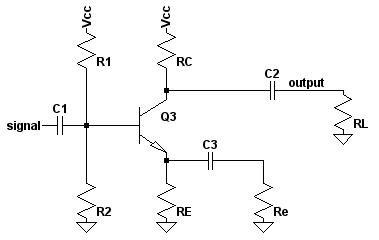
\includegraphics[scale=.6]{teknisk/forforstaerker/ceopkobling.png}
\caption{Generel form på commonemitterkobling med uafkoblet emittermodstand}
\label{fig:cekobling}
\end{figure}


Argumentet for dette valg er at det er det eneste trin, blandt commonemitter, -base og -collector, hvis spændingsforstærkning er betydeligt over én og ikke, under korrekte omstændigheder, afhænger af transistorparametre. Da transistorparametre blandt andet er afhængige af den anvendte transistors temperatur er det en betragtelig styrke ikke at skulle tage højde for dem. Spændingsforstærkningen i commonemittertrinnet er dog kun uafhængig af transistorparametre så længe følgende er gældende: $r_o >>R_C \| R_L$, $gm \cdot R_E||R_e$ og $i_e \approx i_c$.
Dette skyldes at forstærkningen er givet ved ligning (\ref{eq:gmbevis}) \cite{ael-mm6}.

\begin{equation}
A_v =  \frac{-gm \cdot R'_L}{1+gm \cdot R'_e} \approx  -\frac{R'_L}{R'_e} \Biggr\vert _{\frac{1}{gm}<<R'_e}
\label{eq:gmbevis}
\end{equation}

Hvor $R'_e = R_e || R_E$ og $R'_L = R_L||R_C$. Det vil sige at jo tættere $R_e$ kommer på $\frac{1}{gm}$ jo mere indflydelse vil denne have på forstærkningen. Disse antagelser vil derfor være gældende gennem hele designet af forforstærkeren. 

Det første trin skal have en forstærkning på 10 gange og det andet på 6,97 for at opnå den ønskede forstærkning, som vist på figur \ref{blok_forforstaerker}. Grunden til rækkefølgen af trinnene er for ikke at have størst signaludsving og den største forstærkning i samme trin. Dette skyldes at der i en forstærker altid vil være forvrængning og støj. Hvis den største forstærkning kommer sidst, vil denne forvrængning blive forstærket yderligere, hvilket ikke er ønskværdigt. Hvis den største forstærkning derimod kommer først, vil der blive mindst muligt forvrængning med i det endelige signal.\fixme{Hvordan viser vi at det er smart? Frederik: Er det godt nok? Skal der skrives mere? Skal der beregninger med, der beviser det? (synes jeg ikke)}

\begin{figure}[h]
\centering
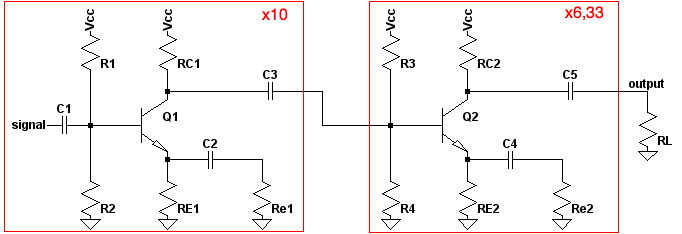
\includegraphics[scale=.6]{teknisk/forforstaerker/blok_forforstaerker.png}
\caption{Blokdiagram over forforstærkerens byggeblokke samt lydsignalets vej}
\label{blok_forforstaerker}
\end{figure}

For at opnå så lav forvrængning som muligt designes hvert trin således at forstærkningen, uden den AC-koblede emittermodstand $R_e$, er så stor som muligt for at gøre tilbagekobling muligt. For derefter at få den ønskede forstærkning tilføjes tilbagekoblingsmodstanden $R_e$.

\subsection*{Design af første trin}
Begge trin designes efter maksimal forstærkning uden $R_e$. Denne forstærkning er givet ved ligning (\ref{eq:dcgain}).

\begin{equation}
|A_{vs}|=\frac{1}{\left(\frac{V_T \cdot R_C}{V_{R_C}}+\frac{R'_S}{\beta}\right) \left(\frac{1}{R_C}+\frac{1}{R_L}\right)}
\label{eq:dcgain}
\end{equation}
Hvor $R'_S = R_S||R_1||R_2$ og $V_T = 26 \cdot 10^{-3}$.

For at designe et kredsløb med maksimal forstærkning justeres størrelsen af $R_C$ uden at variere spændingen over den, $V_{R_C}$. Den maksimale $R_C$ findes ved ligning (\ref{eq:rcmaks}).

\begin{equation}
R_{\mathrm{C,maks}} = \sqrt{\frac{R'_S \cdot R_L \cdot V_{R_C}}{\beta \cdot V_T}}
\label{eq:rcmaks}
\end{equation}

I ligning (\ref{eq:rcmaks}) er $R'_S$ defineret som $R_1||R_2||R_S$. $R_S$ er fastlagt til 2,2 k\ohm, hvilket er mikrofonens udgangsimpedans \cite{mic-datablad}. Parallelforbindelsen mellem $R_1$ og $R_2$ kan ikke beregnes men skal vælges. Indgangsimpedansen i kredsløbet, som netop er $R_1||R_2$, skal som hovedregel være meget større end udgangsimpedansen i den kreds den belaster. En tommelfingerregel siger at 10 gange større er tilstrækkeligt til at være $"$meget større$"$ hvormed parallelkoblingen skal være over eller lig med 22 k\ohm. 
Belastningen, $R_L$, for det første trin bliver indgangsimpedansen i det andet. Indgangsimpedansen i det andet trin bliver $R_3||R_4$ og kan heller ikke beregnes. Da $R_C$ i det første trin ikke kendes endnu vælges indgangsimpedansen i det andet til at være den samme som i det første, altså 22 k\ohm. 
$V_{R_C}$ er defineret som værende $V_{CC} - V_{\mathrm{CE,sat}} - V_{R_E} - V_{\mathrm{o,peak}}$, hvor $V_{CC}$ vælges til 15 V så der sikres at der er plads til det ønskede spændingsudsving, $V_{R_E}$ vælges til 3 V og $V_{\mathrm{CE,sat}}$ aflæses i databladet for BC547b \cite{bc547b-datablad} til 0,2 V ved en collectorstrøm på 1 mA. Der antages at collectorstrømmen cirka bliver 1 mA. Ligeledes aflæses $\beta$ til 250 ved 1 mA i databladet. $V_{\mathrm{o,peak}}$ er peakspændingen på udgangen. Dermed bliver peakspændingen en faktor 10 højere end mikrofonens output peakspænding. $V_{\mathrm{o,peak}}$ bliver derfor 316 mV. $R_{C1}$ beregnes hermed i ligning (\ref{eq:rcforsteberegning}).

\begin{equation}
R_{\mathrm{C1}} = \sqrt{\frac{22~k\ohm || 2,2~k\ohm \cdot (15~V - 0,2~V - 3~V - 0,287~V)}{250 \cdot 26 \cdot 10^{-3}}}=8,83~k\ohm
\label{eq:rcforsteberegning}
\end{equation}

$R_{E1}$ bestemmes i ligning (\ref{eq:beregningre1}) under antagelse at $i_e = i_c$.  $i_c$ beregnes i ligning(\ref{eq:ff:ic}).

\begin{equation}
\label{eq:ff:ic}
i_C=\frac{V_{R_C}}{R_C}=\frac{11,5~V}{9,25~k\ohm}=106,4~mA
\end{equation}
\begin{equation}
R_{E1}=\frac{V_{R_{E1}}}{\frac{V_{R_{C1}}}{R_{C1}}}  \Rightarrow R_{E1}=\frac{3~V}{106,4~mA}=2,30~k\ohm
\label{eq:beregningre1}
\end{equation}


Dernæst beregnes $R_{e1}$ ud fra hvad den ønskede forstærkning skal være. Ligning (\ref{eq:gmbevis}) benyttes til at beregne $R_{e1}$ i ligning (\ref{eq:rlilleeberegning}).

\begin{equation}
\label{eq:rlilleeberegning}
A_v = -\frac{R'_L}{R'_e} \Rightarrow  R_{e1} =-\frac{R_L \cdot R_{C1} \cdot R_{E1}}{A_v \cdot R_{E1} \cdot R_{C1} + A_v \cdot R_{E1} \cdot R_L + R_{C1} \cdot R_L} \Rightarrow R_{e1} = 867,6~\ohm
\end{equation}

Biasnetværket, bestående af $R_1$ og $R_2$ beregnes ud fra den spænding, som er påkrævet på basen for at transistoren fungerer som ønsket. Spændingen over base-emitter, $V_{\mathrm{BE}}$ er i databladet aflæst til 0,6 V. Da potentialet på emitteren er 3 V skal potentialet på basen være 3,6 V. $R_1$ og $R_2$ kan beregnes ud fra at $V_{R_2}$ skal være 3,6 V og parallelkoblingen $R_1||R_2$. Beregningen udføres i ligning (\ref{eq:r1r21}) og (\ref{eq:r1r22}).

\begin{equation}
V_{R_2} = V_{CC} \cdot \frac{R_2}{R_1+R_2} 
\label{eq:r1r21}
\end{equation}
\begin{equation}
R_1||R_2 = \frac{R_1 \cdot R_2}{R_1 + R_2}
\label{eq:r1r22}
\end{equation}
De kendte værdier indsættes og de to ligninger med to ubekendte løses. Resultatet er vist i ligning (\ref{eq:r1r2result}).
\begin{equation}
R_1 = 91,7~k\ohm ~ \wedge ~ R_2=28,9~k\ohm
\label{eq:r1r2result}
\end{equation}

For at opnå den ønskede frekvensgang skal $C1$, $C2$ og $C3$ dimensioneres således at den knækfrekvens de hver især frembringer. Da knækfrekvensen er det punkt hvor kurven er faldet 3 dB og frekvensgangen skal, jævnfør kravspecifikationen, være 20 Hz til 20 kHz, er det nødvendigt at knækfrekvens  ligger før 20 Hz. Det vurderes at knækfrekvensen beregnes til at ligge i 2 Hz for at knækfrekvensen ikke giver anledning til en dæmpning af signalet på mere end de tilladte 3 dB.

Kondensatorerne beregnes med formel (\ref{eq:kondensatorknaek}).

\begin{equation}
C=\frac{1}{\omega \cdot R}=\frac{1}{2\cdot \pi \cdot f \cdot R}
\label{eq:kondensatorknaek}
\end{equation}

I ligning \ref{eq:kondensatorknaek} er $C$ kondensatorens capacitet og $R$ er den impedans kondensatoren ser ind i. 
$C1$ ser ind i forspændingskoblingen i det første forstærkertrin, altså 22 k\Ohm. $C2$ ser ind i den AC-koblede emittermodstand, $Re1$. $C3$ ser ind i forspændingsnetværket i det andet forstærkertrin, altså 22 k\Ohm. Dermed bliver kondensatorernes værdier som følger.

\begin{equation}
C1=3,58~\my F~\wedge ~C2=91,9~\my F~\wedge ~C3=3,58~\my F
\end{equation}



\subsection*{Design af andet trin}
Beregning af andet trin følger samme designprocedure som første trin. Kredsløbet til andet trin er vist på figur \ref{fig:andettrinkreds}.

\begin{figure}[h]
\centering
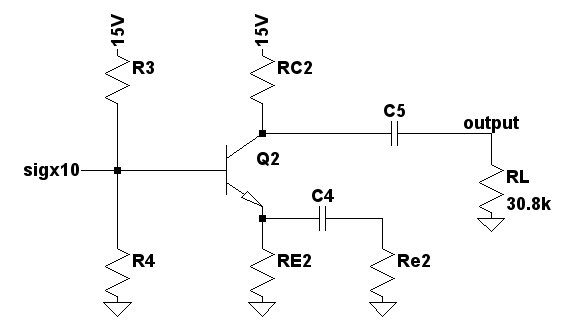
\includegraphics[scale=.6]{teknisk/forforstaerker/andettrinkreds.png}
\caption{Det andet trins kredsløb}
\label{fig:andettrinkreds}
\end{figure}

Det andet trin skal forstærke et signal med en maksimal peakspænding på 287 mV op til 2 V, altså 6,97 gange. Belastningsmodstanden for dette forstærkertrin er bestemt af indgangsvælgeren, som er det næste trin efter forforstærkeren. Indgangsvælgerens indgangsimpedans er 30,8 k\ohm \fixme{reference til indgangsvælgeren hvor det står}. $R_S$ er i dette trin givet ved udgangsmodstanden for det første forstærkertrin, som er lig med $R_{C1}$ hvilket gør at $R'_S = R_{C1} || R_3 || R_4$. Den maksimale $R_{C2}$ beregnes i ligning \ref{eq:rc2maks}.

\begin{equation}
R_{\mathrm{C2}} = \sqrt{\frac{R'_S \cdot R_L \cdot V_{R_C2}}{\beta \cdot V_T}} = 17,1~k\ohm
\label{eq:rc2maks}
\end{equation}

Beregningerne af $R_{E2}$ og $R_{e2}$ samt kondensatorerne er meget ens med dem for det første forstærkertrin. Derfor er det valgt ikke at vise beregningerne i rapporten. $R_3$ og $R_2$ antager samme værdier som henholdsvis $R_1$ og $R_2$, da begge trin skal have samme indgangsimpedans. De beregnede værdier er vist i ligning (\ref{eq:valuestrin2}).

\begin{equation}
R_{E2}=5233,7~\ohm ~ \wedge ~R_{e2}=2599,4~\ohm ~ \wedge ~ C4=30,6~\my F ~ \wedge ~ C5=2,6~\my F
\label{eq:valuestrin2}
\end{equation}

Det endelige kredsløb er vist på figur \ref{fig:forforstaerkersimuleringkredslob} i simuleringsafsnittet.

\subsection*{Simulering}

For at verificere at kredsløbet fungerer som ønsket simuleres det i LTspice. De karakteristika som skal verificeres er spændingsforstærkningen, amplitudekarakteristikken samt harmonisk forvrængning. Kredsløbet der simuleres er vist på figur \ref{fig:forforstaerkersimuleringkredslob}. 

\begin{figure}[h]
\centering
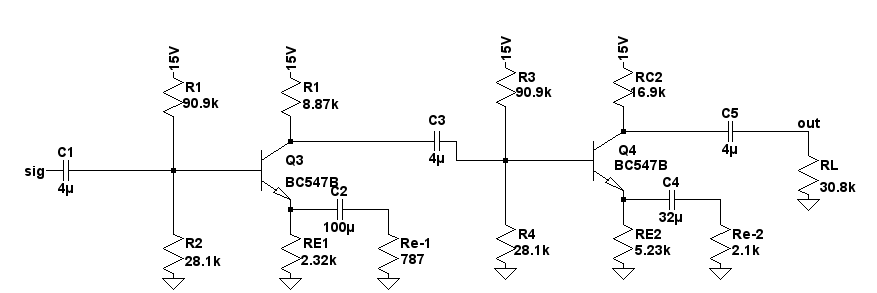
\includegraphics[scale=.6]{teknisk/forforstaerker/forforstaerkerendeligkreds.png}
\caption{}
\label{}
\end{figure}

Spændingsforstærkningen af hele trinnet skal være 69,7 gange svarende til 36,9 dB. Forstærkningen vises på figur \ref{fig:amplitude-forforstaerker} ved hjælp af en amplitudekarakteristik, således at spændet fra 20 Hz til 20 kHz tydeligt kan ses. 


\begin{figure}[h]
\centering
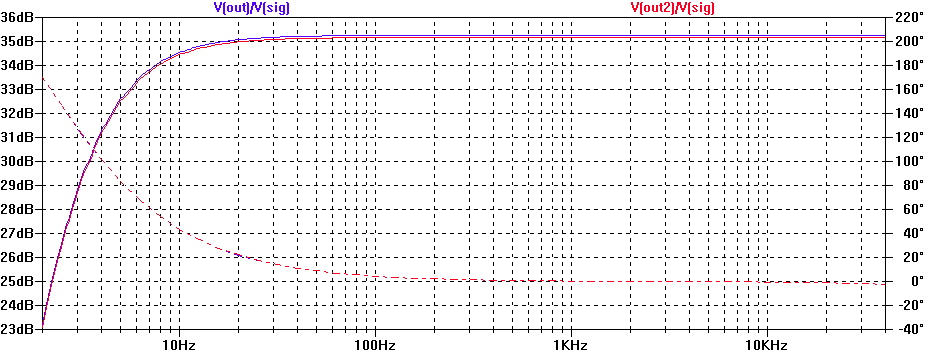
\includegraphics[scale=.6]{teknisk/forforstaerker/amplitudeforforstaerker.png}
\caption{Forforstærkerens amplitude karakteristik}
\label{fig:amplitude-forforstaerker}
\end{figure}

Simuleringen viser at forstærkningen ved 1 kHz, som er referencen jævnfør kravspecifikationen, er 36 dB hvor den skulle have være 36,9 dB. Dermed må der konkluderes at beregningen af forforstærkertrinnene indeholder usikkerheder. Usikkerhederne vurderes til at bestå i de antagelser som defineres før beregningerne: $r_o >>R_C \| R_L$, $gm \cdot R_E||R_e$ og $i_e \approx i_c$. For at korrigere forstærkningen i trinnene kan der, ifølge ligning \ref{eq:gmbevis}, justeres på den AC-koblede emittermodstand, $R_{e1}$ og $R_{e2}$. I ligning \ref{eq:nyerevalues} er de nye værdier for disse modstande anvist. Modstandsværdierne er fundet ved først at justere $R_{e1}$ til det første trin giver den korrekte forstærkning for derefter at gøre det samme med det andet trin.

\begin{equation}
R_{e1}=790~\ohm~\wedge ~R_{e2}=2,1~k\ohm
\label{eq:nyerevalues}
\end{equation}

Med de nye modstandsværdier bliver amplituden som vist på figur \ref{fig:rigtigamplitudeforforstaerker}.

\begin{figure}[h]
\centering
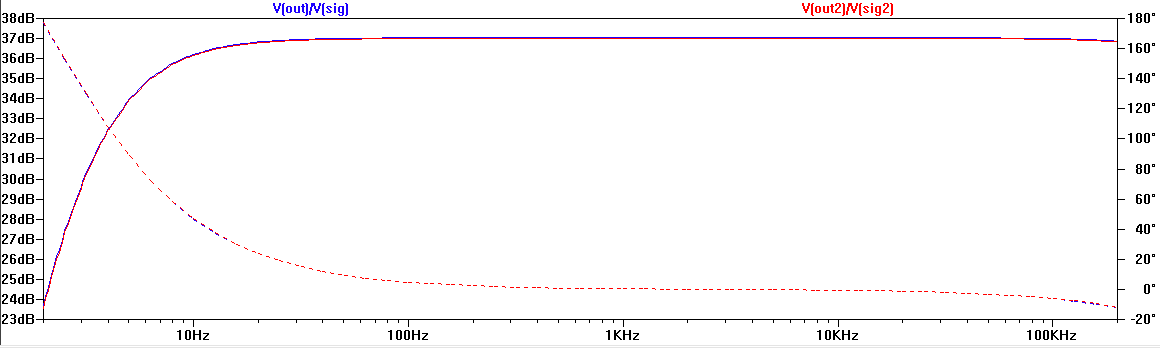
\includegraphics[scale=.6]{teknisk/forforstaerker/rigtigamplitude.png}
\caption{Forforstærkerens amplitudekarakteristik efter korrektion af forstærkning}
\label{fig:rigtigamplitudeforforstaerker}
\end{figure}

På figur \ref{fig:rigtigamplitudeforforstaerker} ses det at forstærkningen nu er korrigeret. Derudover fremgår det at dæmpningen fra 20 kHz til 20 Hz er 0,2 dB. Dermed overholdes kravet om at dæmpningen i dette område, som skal være under 0,375 dB. 

Den harmoniske forvrængning skal ifølge kravspecifikationen være under 0,5 \%. Ifølge LTspice er den harmoniske forvrængning ved 1 kHz og maksimal peakspænding på indgangen 0,18 \%. Forvrængningsmålingen er udført ved maksimal peakspænding da forvrængningen i trinnet vil være mest kritisk i den situation. 








\section{Indgangsvælger}
\begin{frame}{Indgangsvælger - Krav}
\scriptsize{
\begin{table}[h]
\centering
\begin{tabular}{l|r}
\hline\hline
Område & Krav \\
\hline\hline
Antal trin i & 4 \\
indgangsvælgeren & \\[4pt]
Indgangsimpedans & \> 22 k\ohm \\[4pt]
Frekvensgang & \< 0,375 dB ved 20 Hz - 20 kHz, ref. 1 kHz \\
& \< 0,75 dB fra 20 Hz til 63 Hz \\
& \< 0,75 dB fra 12,5 kHz til 20 kHz \\[4pt]
Dæmpning af slukket & \> 50 dB ved 1 kHz \\
indgangssignal & \\
\hline\hline
\end{tabular}
\label{tab:krav_indgangsvaelger}
\end{table}
}
\end{frame}

\begin{frame}{Indgangsvælger - Opbygning}

\begin{figure}[h]
\centering
\includegraphics[width=\textwidth]{../rapport/teknisk/indgangsvaelger/signal-taend-sluk.png}
\label{fig:indgangsvaelger-overordnet}
\end{figure}
\end{frame}

\begin{frame}{Indgangsvælger - Styring}

\begin{figure}[h]
\centering
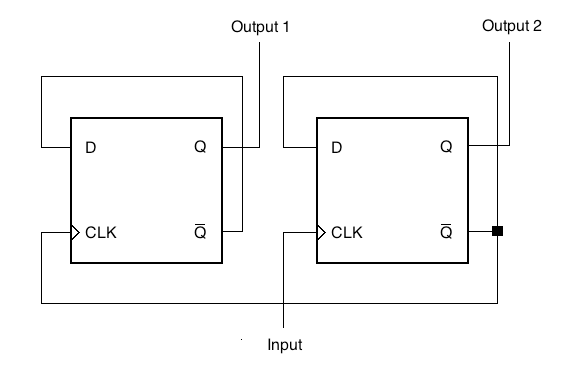
\includegraphics[scale=0.4]{../rapport/teknisk/indgangsvaelger/flipflop.png}
\label{fig:indgangsvaelger-flipflop}
\end{figure}
\end{frame}

\begin{frame}{Indgangsvælger - Simulering}
\begin{figure}[h]
\centering
\includegraphics[width=\textwidth]{../rapport/teknisk/indgangsvaelger/simulering/frekvenskarakteristik.png}
\label{indgangsvaelger_frekvenskarakteristik}
\end{figure}
\end{frame}

\begin{frame}{Indgangsvælger - Måling}
\begin{figure}[h]
\centering
\includegraphics[width=\textwidth]{../rapport/maalerapporter/indgangsvaelger/Indgangsvlger-mic-200mv-frek.png}
\label{fig:indacc:frek200mv}
\end{figure}
\end{frame}

\begin{frame}{Indgangsvælger - Måling}
\begin{figure}[h]
\centering
\includegraphics[width=\textwidth]{../rapport/maalerapporter/indgangsvaelger/Indgangsvlger-mic-2v-thd.png}
\label{fig:accind:thd2v}
\end{figure}
\end{frame}


\begin{frame}{Indgangsvælger - Oversigt}
\scriptsize{
\begin{table}[h]
\centering
\begin{tabular}{l|r|r}
\hline\hline
Område & Krav & Status \\
\hline\hline
Antal trin i & 4 & \checkmark \\
indgangsvælgeren & \\[4pt]
Indgangsimpedans & \> 22 k\ohm & \checkmark \\[4pt]
Frekvensgang & \< 0,375 dB ved 20 Hz - 20 kHz, ref. 1 kHz & \checkmark \\
& \< 0,75 dB fra 20 Hz til 63 Hz & \checkmark\\
& \< 0,75 dB fra 12,5 kHz til 20 kHz & \checkmark\\[4pt]
Dæmpning af slukket & \> 50 dB ved 1 kHz & \checkmark \\
indgangssignal & \\
\hline\hline
\end{tabular}
\label{tab:krav_indgangsvaelger}
\end{table}
}
\end{frame}
\subsection*{Beregninger}

\begin{figure}[h]
\centering
\includegraphics[scale=0.4]{teknisk/indgangsvaelger/signal-taend-sluk.png}
\caption{Opbygning af indgangsvælgeren}
\label{indgangsvaelger-overordnet}
\end{figure}

Modstandene $R_1$ og $R_2$ er begge valgt til 100k\ohm, for at give et DC-offset på ca 2.5V, halvdelen af V1. Dette gælder dog kun når transistoren er slukket. I det transistoren tændes, sættes $R_2$ parallelt med $R_3$, hvilket trækker DC-offsettet længere ned:
\begin{equation}
5V\cdot \frac{\frac{1}{\frac{1}{R_2}+\frac{1}{R_3}}}{R_1+\frac{1}{\frac{1}{R_2}+\frac{1}{R_3}}}=1.11 V
\end{equation}
Dog er det egentlige DC-offset underordnet, så længe det ligger indenfor et område transistoren kan arbejde med, og DC-offset $-$ AC-Peakværdi $>$ 0 når transistoren er slukket. DC-offsettet alligevel bliver filtreret fra gennem en kondensator, før summationsforstærkeren, så det ikke har indflydelse på det endelige signal.
Modstanden $R_3$ er valgt ud fra, at signalet skal se en indgangsimpedans på minimum 22 k\ohm. Når transistoren er tændt er indgangsimpedansen mindst. $R_1$, $R_2$ og $R_3$ sidder så alle parallelt hvilket giver:
\begin{equation}
\frac{1}{\frac{1}{R_1}+\frac{1}{R_2}+\frac{1}{R_3}}=22 k\ohm
\\
R_3=39.29 k\ohm
\end{equation}
Denne er så valgt til 40.2k\ohm, for at passe med E96-rækken.
For at kunne afbryde de enkelte signaler, kan transistoren Q1 trække signalet til stel. for at tillade at hele signalet bliver trukket til stel, skal hele den strøm der løber igennem systemet føres ned igennem transistoren. Den maksimale strøm der kan løbe i systemet er summen af DC-strømmen og AC-strømmen. 
Først findes DC-strømmen. DC spændingen i kredsløbet er sat til 5V. Hvis transistoren en direkte kobling, så der ligger stel mellem $R_3$ og $R_4$, vil $R_2$ og $R_3$ sidde i parallel til stel. Ud fra dette findes den maksimale mængde strøm, der kan løbe igennem $R_3$. Ud fra dette den største strøm der vil løbe igennem $R_3$, og derfor også transistoren, udregnes til ca. 0.027 mA
Den maksimale AC-strøm findes ved at kortslutte alle kondensatorer, og regne med det størst mulige AC-udsving. En konsekvens af, at alle kondensatorer bliver kortsluttet, er at forsyning og stel også bliver kortsluttet. Ud fra dette findes AC-strømmen til at være ca. 0.05 mA. Dette giver en samlet max strøm på ca. 0.08 mA.
Strømmen $I_B$, som løber ind i basis på transistoren skal mindst være den samlede strøm, divideret med $H_{FE}$. $H_{FE}$ er aflæst til 200:
\begin{equation}
I_B = \frac{0.08 mA}{H_{FE}} = 0.004 mA
\end{equation}
Da de benyttede flip-flops\fixme{Check at det stadig er sådan} outputter 5 V, kan $R_B$'s maksimale værdi findes. Der skal dog tages højde for at der ligger en diodestrækning mellem basis og emitter:
\begin{equation}
R_B = \frac{5 V-0.6V}{I_B} =  11M\ohm
\end{equation}
Alt under dette vil give en større strøm ind i basis, hvilket vil give en større strøm ind i collectorbenet og vil derfor også kunne trække signalet til stel.
Modstanden $R_4$ har ikke nogen indvirkning på indgangsimpedansen når transistoren er tændt og signalet derfor er slukket. Den er valgt til 40.2 k\ohm, det samme som $R_3$, for at gøre produceringen enklere. Ved at bruge modstande med de samme værdier sænkes antallet af benyttede komponenter, hvilket letter indkøbs- samt produceringsomkostninger. Når signalet er tændt, sidder den i serie med $R_3$, hvilket giver en højere indgangsimpedans:
\begin{equation}
R_{indgang}=\frac{1}{\frac{1}{R_1}+\frac{1}{R_2}+\frac{1}{R_3+R_4}}=30.8 k\ohm
\end{equation}

Efter at have opstillet de forskellige modstandsværdier, er det muligt at udregne værdien af afkoblingskondensatorerne i kredsløbet. Disse kan udregnes som en spændingsdeling mellem en seriekoblet modstand og kondensator, seriekoblet med en modstand, som vist på figur \ref{crvd}. I dette tilfælde vil $R_U$ være udgangsimpedansen på det foregående led, og $R_I$ være indgangsimpedansen på det efterfølgende. Impedansen i en kondensator, i frekvensdomænet er $\frac{1}{s\cdot C}$. Dette kan opstilles i følge spændingsdelingsformel for udregningen:
\begin{equation}
\frac{V_{out}}{V_{in}}=\frac{R_I}{R_I+(R_U+\frac{1}{s\cdot C})}
\end{equation}
For at få en dæmpning på 3dB, som er den ønskede dæmpning i knækpunktet, skal $\frac{V_{out}}{V_{in}}=10^{\frac{-3}{20}}\approx0.7$. 
Dette giver 2 ubekendte, s og C. s kan ses som $2\cdot \pi \cdot f$, hvor f er den ønskede frekvens ved knækket. Der opstilles et udtryk for C:
\begin{equation}
10^{\frac{-3}{20}}=\frac{R_I}{R_I+(R_U+\frac{1}{2\cdot\pi\cdot 2\cdot C})}\\
C=\frac{-1}{2}\cdot{10^{\frac{-3}{20}}}{\pi\cdot f\cdot(10^{\frac{-3}{20}}\cdot R_I+\frac{-3}{20}}\cdot R_U - R_I)
\end{equation}
f bestemmes til 2hz, én dekade før den ønskede, for at opnå en lav dæmpning ved de ønskede 20hz. Ud fra dette kan de forskellige værdier for C udregnes, afhængigt af de impedanser de ser ind i.
Indgangsimpedansen for $C_1$ er fundet til 30.8 k\ohm . Indtastes dette i ovennævnte formel findes værdien for $C_1$ til mindst 8µF. Alt under dette vil give en højere knækfrekvens, hvilket ikke er at ønske. Alt højere vil dog give en større indsvingningstid, hvilket er at foretrække, dog heller ikke ønskeligt.
\subsection{Simulering}
Efter at indgangsvælgeren er blevet designet og beregnet, er der lavet en række simuleringer for se om kredsløbet opfører sig som ønsket og, hvis der er afvigelser, give en begrundelse for hvorfor. I dette afsnit vil der blive simuleret følgende; dæmpning af signal, THD, frekvenskarakteristik, forstærkning i kredsløbet og tænd og sluk af signal. Det samlede diagram der er simuleret kan ses på figur \ref{diagram_simulering}. 

\begin{figure}[h]
\centering
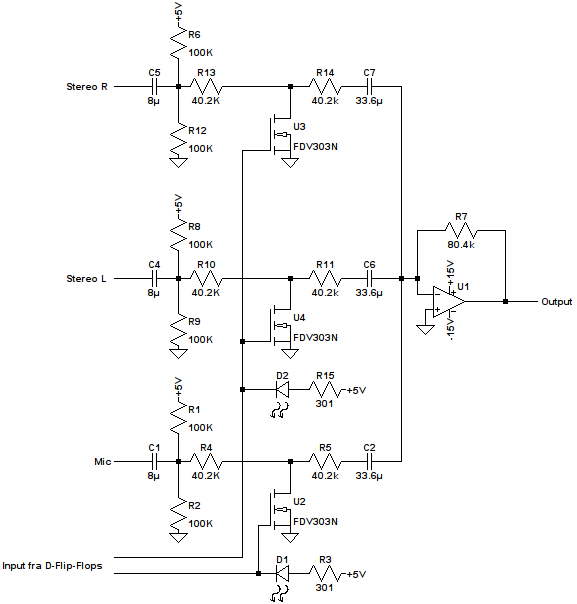
\includegraphics[scale=0.8]{teknisk/indgangsvaelger/simulering/indgangvaelger_ltspice_diagram.png}
\caption{Diagram over det kredsløb der simuleres.}
\label{diagram_simulering}
\end{figure}

\subsubsection*{Forstærkning i kredsløbet}
Fra beregningerne vides det at kredsløbet er designet til at have en forstærkning på 1. Derudover vil signalet efter indgangsvælgeren også være inverteret fordi der bruges en inverterende forstærker til at summere signalerne. Det simulerede signal er vist på figur \ref{indgangsvaelger_input/output}. Simuleringen er lavet ved en transient analyse over 3 ms, med en maksimum timestep på 0,01 µs og en peakspænding på 2 V 1 kHz på indgangen. På figur \ref{indgangsvaelger_input/output} ses det at forstærkningen på 1 ikke helt er opnået, det skyldes at generatoren har en udgangsmodstand på 2,2 k\ohm. Signalet er inverteret som forventet. 
\begin{figure}[h]
\centering
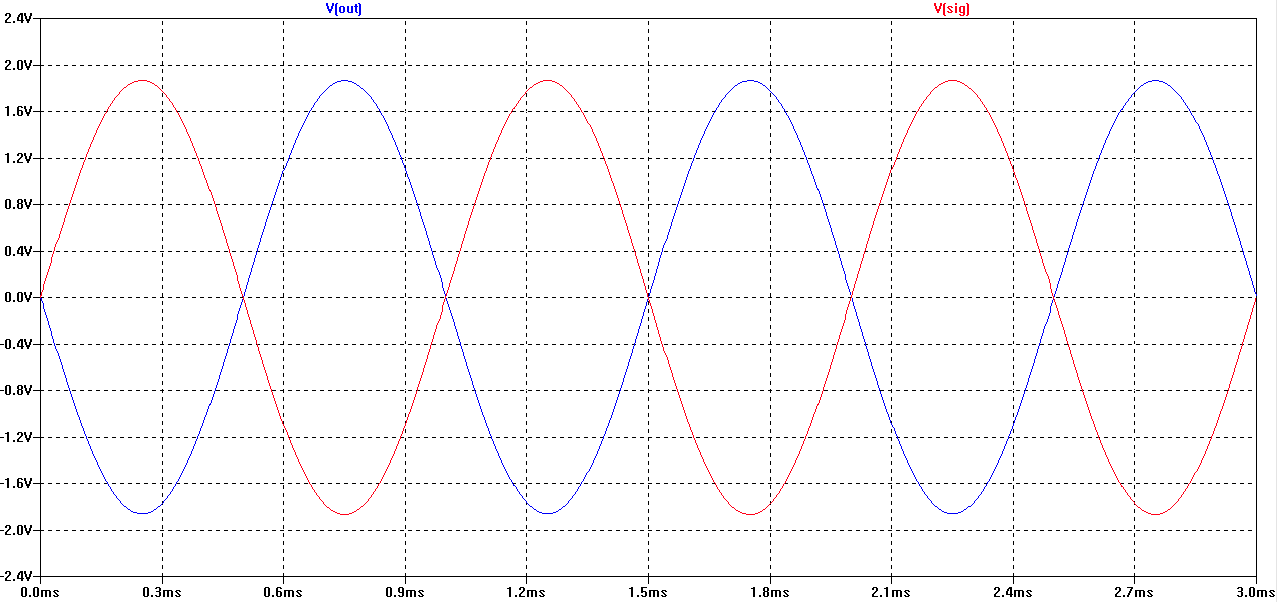
\includegraphics[width=\textwidth]{teknisk/indgangsvaelger/simulering/input_output.png}
\caption{Simuleret forstærkningen igennem indgangsvælgeren, hvor den røde kurve er inputsignalet til indgangsvælgeren og den blå er outputsignalet fra indgangsvælgeren}
\label{indgangsvaelger_input/output}
\end{figure}

\subsubsection*{Frekvenskarakteristik}
På figur \ref{indgangsvaelger_frekvenskarakteristik} er simuleringen af frekvenskarakteristikken vist. Simuleringen er lavet ved en AC-Analyse fra 2 Hz til 200 kHz, og ved at sætte output over input ved 0 V på transistoren. Fra tabel \ref{tab:krav_indgangsvaelger} er der opsat krav om frekvensområdet. På simuleringen ses det at fra 10 kHz til 20 kHz er der en lille afvigelse på ca. 0,06 dB. Afvigelsen skyldes at transistoren der er brugt har en passiv kapacitet, der gør at ved høje frekvenser vil signalet falde af.

\begin{figure}[h]
\centering
\includegraphics[width=\textwidth]{teknisk/indgangsvaelger/simulering/frekvenskarakteristik.png}
\caption{Simuleret frekvens- og fasekarakteristikken for indgangsvælgeren}
\label{indgangsvaelger_frekvenskarakteristik}
\end{figure}

\subsubsection*{Dæmpning af signal}
På figur \ref{indgangsvaelger_daempniing} ses en graf over den simulerede dæmpning i kredsløbet. Simuleringen er lavet ved en AC-Analyse fra 2 Hz til 200 kHz, og ved at sætte output over input ved 5 V på transistoren. Fra kravspecifikationen er der opsat krav om at isoleringen af signaler skal være større end 50 dB, hvilket altså opnåes i simuleringen.
\begin{figure}[h]
\centering
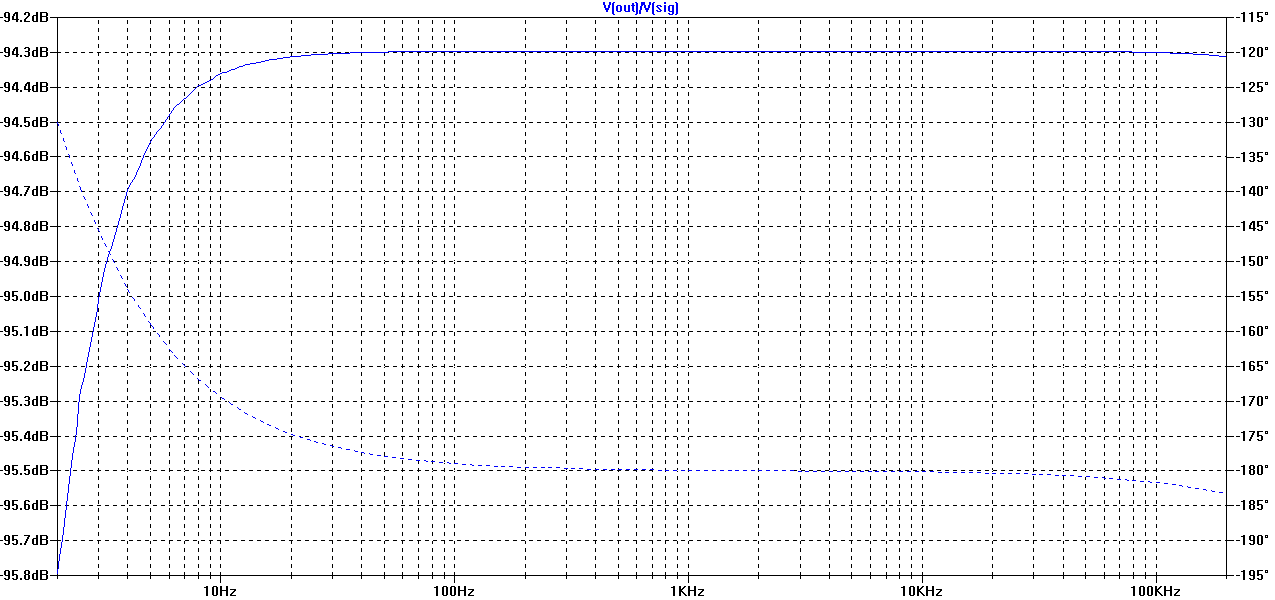
\includegraphics[width=\textwidth]{teknisk/indgangsvaelger/simulering/daempning_af_signal.png}
\caption{Dæmpningsgraden af signalet, når det er slukket.}
\label{indgangsvaelger_daempniing}
\end{figure}
\fixme{Ret den jf. Jans kommentarer}

\subsubsection*{Tænd og sluk af signal}
På figur \ref{indgangsvaelger_taendsluk} er der simuleret at et signal bliver tændt og slukket. Simuleringen er lavet ved en transient analyse over 1,4 s, med en maksimum timestep på 0,1 µs og en peakspænding 2 V ved 100 Hz på indgangen. Først er signalet slukket i 100 ms, dernæst er signalet tændt i 700 ms og til sidst er signalet slukket i 600 ms. Som det ses er signalet når det bliver tændt først oppe på niveau efter det har været tændt i 700 ms. Det skyldes at der er brugt kondensatorer i kredsløbet, hvilket giver en længere indsvingningstid.\fixme{Jesper: Der skal ses på hvad denne graf egentlig betyder}
\begin{figure}[h]
\centering
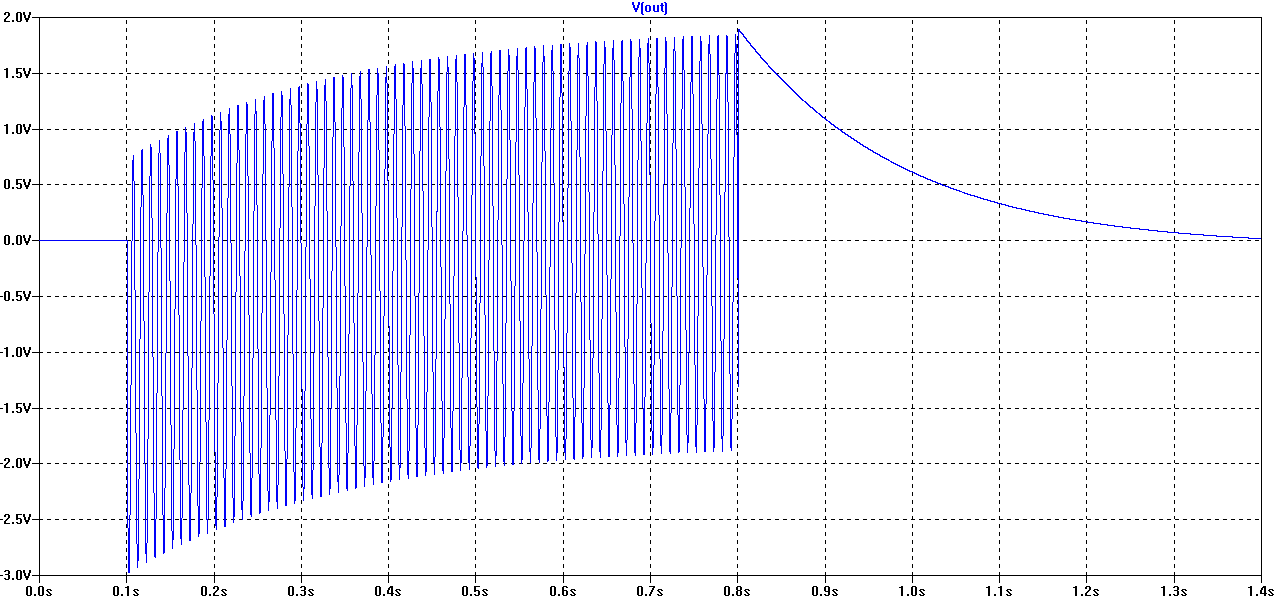
\includegraphics[width=\textwidth]{teknisk/indgangsvaelger/simulering/taend_sluk.png}
\caption{Simulering af at tænde og slukke signalet.}
\label{indgangsvaelger_taendsluk}
\end{figure}

\subsubsection*{THD}
Simuleringen er lavet ved en fourier-analyse og giver en THD på 0,062 \%. Der er dog ikke noget sammenligningsgrundlag fra beregningerne, hvormed der først kan laves udtalelser på denne værdi under accepttesten.

\section{Accepttest}
Indgangsimpedansen for alle indgange gav samme resultat ved målingerne. Indgangsimpedansen, for et slukket og et tændt signal, er, som vist i Appendiks \ref{maalejournal_indgangsvaelger}, henholdsvis 22,62 k\ohm~ og 31,56 k\ohm . Da disse begge er over 22 k\ohm~samt stemmer overens med beregningerne, indenfor komponenttolerancerne, er indgangsimpedansen acceptabel.

Frekvensgangen for 200 mV og 2 V inputspænding, er meget éns, derfor tages der kun udgangspunkt i den ene. Det er valgt at konkludere på frekvensgangen for 200 mV, da denne giver det største udsving. En graf over de målte data kan ses på figur \ref{fig:indacc:frek200mv}.
\begin{figure}[h]
\centering
\includegraphics[width=\textwidth]{maalerapporter/indgangsvaelger/Indgangsvlger-mic-200mv-frek.png}
\caption{Målt frekvensgang for mikrofonindgangen på indgangsvælgeren ved 200 mV inputspænding}
\label{fig:indacc:frek200mv}
\end{figure}

Dæmpningen af et tændt signal ved referencefrekvensen, 1 kHz, er i målingen aflæst til 0,034 dB. Den frekvens som afviger mest fra denne værdi er ved 20 kHz, som aflæses til en dæmpning på 0,13 dB. Dette giver en afvigelse på ca. 0,1 dB, hvilket er meget tæt på det simulerede og under det opstillede krav på 0,375 dB. Dette er derfor acceptabelt.

Målingerne viser, på figur \ref{fig:indaccept:slukketmaaling}, at dæmpning ved 1 kHz er på ca. 114 dB. Denne dæmpning er større end det opstillede krav på 50 dB og er derfor accepteret.
\begin{figure}[h]
\centering
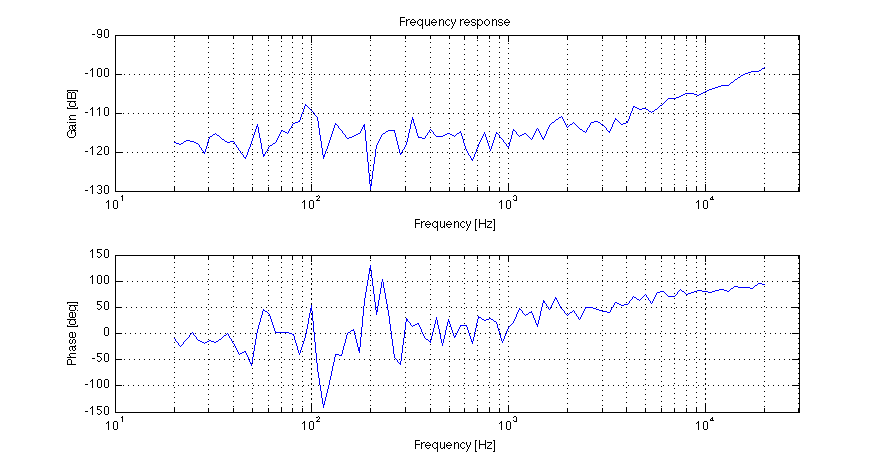
\includegraphics[width=\textwidth]{maalerapporter/indgangsvaelger/Indgangsvlger-mic-2v-slukket-frek.png}
\caption{Frekvensgangen og fasedrejet for mikrofonindgangen for et slukket signal, på indgangsvælgeren ved 2 V. Disse målinger er sandsynligvis støj, da spændingerne er på et meget lavt niveau}
\label{fig:indaccept:slukketmaaling}
\end{figure}	

THD simuleres til 0,062 \% ved en peakspænding på 2 V, ved 1 kHz. Ved en THD måling, illustreret på figur \ref{fig:accind:thd2v}, aflæses THD'en ved 1 kHz til 0,1 \%. 
\begin{figure}[h]
\centering
\includegraphics[width=\textwidth]{maalerapporter/indgangsvaelger/Indgangsvlger-mic-2v-thd.png}
\caption{Målt THD for mikrofonindgangen på indgangsvælgeren ved 2 V inputspænding}
\label{fig:accind:thd2v}
\end{figure}
Det kan dog konkluderes at THD ikke er lav nok. Dette kan delvist løses ved at benytte en anden operationsforstærker, f.eks. OPA27 i stedet for LM324. Det er dog tydeligt, ud fra Appendiks F, at transistorerne ikke afbryder helt, når signalet ikke skal slukkes og at de derfor har en indflydelse. Dette er ikke optimalt og det ville derfor være bedre at benytte en transistor, som afkobler bedre i slukket tilstand.

\begin{table}[h]
\centering
\begin{tabular}{l|r|r}
\hline\hline
Område & Krav & Status \\
\hline\hline
Antal trin i & 4 & \checkmark \\
indgangsvælgeren & \\[4pt]
Indgangsimpedans & > 22 k\ohm & \checkmark \\[4pt]
Frekvensgang & < 0,375 dB ved 20 Hz - 20 kHz, ref. 1 kHz & \checkmark \\
& < 0,75 dB fra 20 Hz til 63 Hz & \checkmark\\
& < 0,75 dB fra 12,5 kHz til 20 kHz & \checkmark\\[4pt]
Dæmpning af slukket & > 50 dB ved 1 kHz & \checkmark \\
indgangssignal & \\
\hline\hline
\end{tabular}
\caption{Oversigt over status af krav til indgangsvælgeren}
\label{tab:krav_indgangsvaelger}
\end{table}

\chapter{Volumenkontrol}
\label{volumenkontrol}

\section{Design}
\label{volumenkontrol-design}

\begin{figure}[h]
\centering
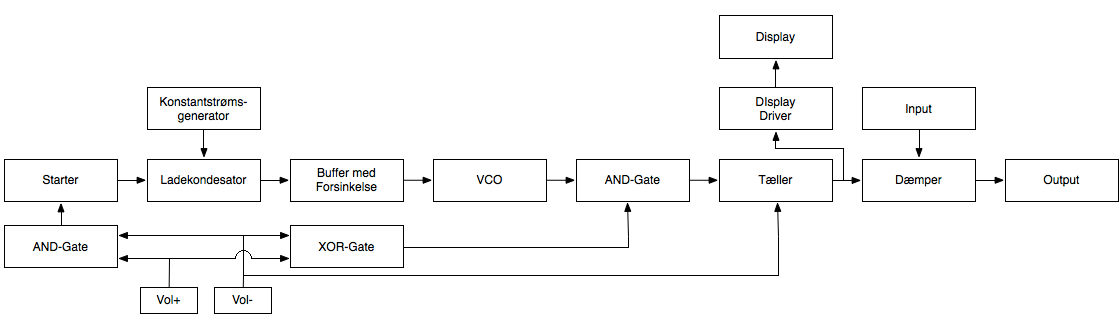
\includegraphics[width=\textwidth]{teknisk/volumenkontrol/blokdiagram.png}
\caption{Blokdiagram over volumenkontrollen}
\label{fig:volumenkontrol_opbygning}
\end{figure}

\section{Simulering}
\label{volumenkontrol-simulering}

\begin{figure}[h]
\centering
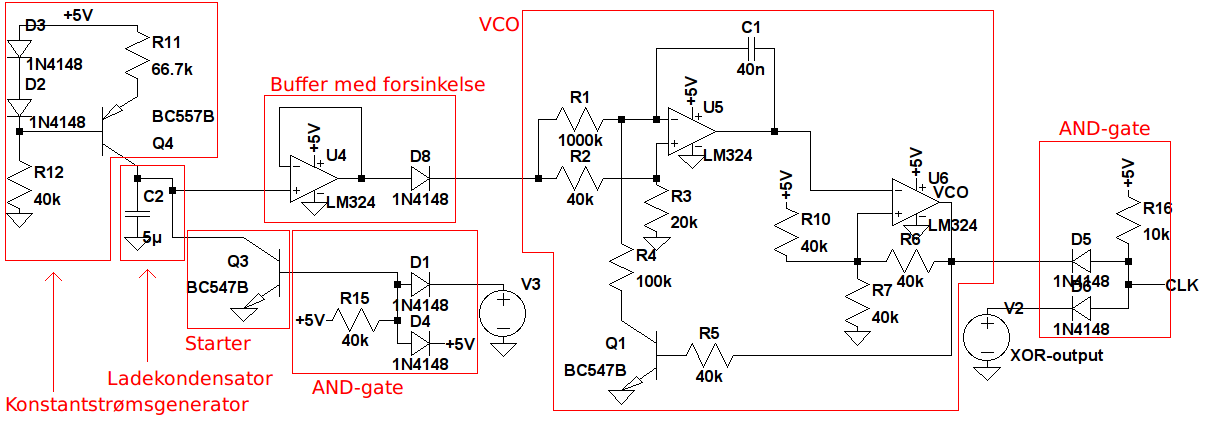
\includegraphics[width=\textwidth]{teknisk/volumenkontrol/diagram.png}
\caption{Diagram over volumenkontrollen}
\label{fig:volumenkontrol_diagram}
\end{figure}

\subsection{Konstantstrømsgenerator}
\label{volumenkontrol-simulering-konstantstroemsgenerator}

Konstantstrømsgeneratorens opgave er at levere en konstant strøm, denne strøm bruges til at oplade en kondensator (ladekondensatoren). Når en kondensator lades med en konstant strøm, vil spændingen over den stige lineært, dette fremgår også af ligning \ref{equ:konstantstroemsgenerator1}.

\begin{equation}
\label{equ:konstantstroemsgenerator1}
V = \frac{I \cdot t}{C}
\end{equation}

Konstantstrømsgeneratoren er designet med udgangs på at der vil være et spændingsfald på 0,5 V over $D_2$, $D_3$, $R_{11}$ og $Q_{4_{BE}}$. I databladet for 1N4148 fremgår det at den vil have en $V_D$ spændingen på 0,5 V ved en $I_F$ strøm på 0,1 mA. Strømmen igennem dioderne er givet ved den strøm, der vil løbe igennem det der kommer efter dem, i dette tilfælde modstanden $R_{12}$. $R_{12}$ er således givet ved ligningen \ref{equ:konstantstroemsgenerator2}.

\begin{equation}
\label{equ:konstantstroemsgenerator2}
R_{12} = \frac{V_{CC} - 2 \cdot V_D}{I_F} = \mathrm{\frac{5~V - 2 \cdot 0,5~V}{0,1~mA} = 40~k\ohm}
\end{equation}

Da der nu ligger en konstant spænding over alle dioderne, kan man se dioden i transistoren som siddende parallelt, med det samme spændingsfald som $D_2$. Dette giver at der findes det samme, konstante, spændingsfald over $D_3$ og $R_{11}$, hvilket giver en konstant strøm gennem $R_{11}$.
Den kondensator som konstantstrømsgeneratoren kaldes ladekondensatoren, denne har en kapacitet på 5 $\mu\mathrm{F}$ og den ønskede oplade tid er 3 s. Kondensatoren oplades fra 0 V til $V_{CC} - V_D$ = 4,5 V, hvor $V_D$ er spændingen over én diode. Udfra disse to ting kan den konstante strøm, $I_{konst}$, nu beregnes, se ligning \ref{equ:konstantstroemsgenerator3}.

\begin{equation}
\label{equ:konstantstroemsgenerator3}
V_{CC} - V_D = \frac{I_{konst} \cdot t}{C} \Rightarrow 4,5~V = \frac{I_{konst} \cdot 3~s}{5~\mu F} \Rightarrow I_{konst} = 7,5~\mu A
\end{equation}

Spændingen over $R_{11}$ er, som tidligere nævnt, 0,5 V og strømmen igennem den er $I_{konst}$, der kan Ohms lov bruges til at beregne modstanden, se ligning \ref{equ:konstantstroemsgenerator4}.

\begin{equation}
\label{equ:konstantstroemsgenerator4}
V_D = R \cdot I_{konst} \Rightarrow 0,5~ V = R \cdot 7,5~\mu A \Rightarrow R = 66,7~k\ohm
\end{equation}

\subsection{Starter}
\label{volumenkontrol-simulering-starter}

Starterens opgave er at holde spændingen over ladekondensatoren på 0 V, når der ikke trykkes på en af volumenknapperne. Dette gøres ved at lede al den strøm som konstantstrømsgeneratoren leverer til stel. Så snart der trykkes på en af volumenknapperne, vil basis på transistoren blive trukket lav, hvilket vil afbryde collector-emitter strømmen. Dette gøres for at sikre at ladekondensatoren er klar til at starte opladningen med det samme.
\subsection{Buffer med forsinkelse}
\label{volumenkontrol-simulering-buffer}

Bufferen sikrer at ladekondensatoren bliver lineært opladet, dette gøres ved ikke at belaste konstantstrømsgeneratoren eller ladekondensatoren. Forsinkelsen laves ved hjælp af en diode. Dioden forsinker signalet ved blot at have et spændingsfald over den, det betyder at spændingen først skal vokse op til minimum en diodespænding, før der kommer en kontrolspænding til VCO'en. Forsinkningen er derfor direkte afhængig af diodespændingen. Dette betyder, at der for at kunne indstille på forsinkelsesperioden skal indsættes en anden diode, med en anden $V_{D}$; eksempelvis en eller flere germaniumsdioder.

\subsection*{VCO}
\label{volumenkontrol-design-vco}

En VCO, Voltage Controlled Oscillator, leverer et konstant signal hvor frekvensen er afhængig af en kontrolspænding. Kontrolspændingen er spændingen over $C_2$, ladekondensatoren, minus én diodespænding. Der er taget udgangspunkt i en VCO fra databladet for en LM324. VCO'en kan deles op i to blokke; én integrator og én schmidt-trigger. Det er udgangen fra schmidt-triggeren der bestemmer hvilken af de to spændinger integrator arbejder udfra. Triggerspændingerne på schmidt-triggeren er givet ved ligning (\ref{equ:vco1}) og (\ref{equ:vco2}). Forsyningsspændingen, $V_{CC}$, er 5 V.

\begin{equation}
\label{equ:vco1}
V_L = \frac{1}{3} \cdot V_{CC} = 1,67~\mathrm{V}
\end{equation}

\begin{equation}
\label{equ:vco2}
V_U = \frac{2}{3} \cdot V_{CC} - 0,5~\mathrm{V} = 2,83~\mathrm{V}
\end{equation}

Frekvensen VCO'en vil svinge med, er givet ved ligning (\ref{equ:vco3}), udtrykket er udledt i appendiks A??.

\begin{equation}
\label{equ:vco3}
f = \frac{1}{\frac{2 \cdot V_{CC} \cdot C \cdot R_1^2}{3 \cdot V_C \cdot (R_1 - R_4)}} = \frac{3 \cdot V_C \cdot (R_1 - R_4)}{2 \cdot V_{CC} \cdot C \cdot (R_1)^2}
\end{equation}

Forholdet mellem høj og lav, duty-cyclen, er givet ved forholdet mellem $R_1$ og $R_4$, i dette tilfælde $\frac{R_4}{R_1} = \frac{40~k\ohm}{80~k\ohm}=0.1$. Dette skyldes at det er disse to modstande $C_1$ op- og aflades igennem. Formlen er udledt i appendiks A??. Grunden til at frekvensen stiger når spændingen stiger, er at opampen altid vil presse sine indgange til at være ens. Da der på plus-indgangen sidder en spændingsdeling, som giver halvdelen af styringsspændingen, vil der ligge det samme på minus-benet. Dette betyder, at spændingsfaldet over $R_1$ altid vil være halvdelen af styringsspændingen. Dette vil betyde at der vil løbe en strøm igennem $R_1$ ind i kondensatoren. Når transistoren leder, vil den lede strømmen, som løber igennem $R_1$ samt den strøm der kommer fra kondensatoren. Når kondensatoren aflader igennem transistoren vil den prøve at trække minus benet ned. Dette prøver op-ampen at undgå ved at øge output spændingen. Hvis man lader denne proces fortsætte uendeligt vil plus- og minus-benet være ens, indtil op-ampen rammer sin maksimale spænding. Herefter vil den ikke være i stand til at regulere spændingen på minus-benet, hvilket vil resultere i at spændingen på minus-benet vil være spændingsdelingen mellem $R_1$ og $R_4$. Dette forhindrer Schmidt-triggeren dog, ved at ændre på hvor strømmen igennem $R_1$ har mulighed for at løbe hen. Når der løber strøm til minus-benet vil dette føre til en spændingstigning. Da op-ampen stadig vil forsøge at holde indgangene éns, vil dette betyde et spændingsfald på outputtet. Det er denne effekt der gør svingningen mulig.

Outputtet fra Schmidt-triggeren er højt, som standard, da outputtet fra integratoren, når denne ikke har en høj nok styringsspænding til at gå i gang, vil være lavt. Dette betyder at AND-gaten der giver signalet videre til tælleren kan give et positivt output, når en knap trykkes ned en enkelt gang. På denne måde vil det være muligt benytte knapperne til at regulere et enkelt niveau op eller ned, samtidig med muligheden for at holde dem inde, og aktivere VCO'en, for at regulere volumeniveauet hurtigere.


%Denne strøm kan kun løbe ind i kondensatoren, hvilket vil oplade denne. Når kondensatoren aflades gennem $R_4$ vil minusbenet gå mod en lavere spænding. For at undgå dette vil op-ampen outputte en højere spænding, for at forsøge at holde begge input på samme spændingsniveau. Kondensatoren blev ved med at aflade, ville op-ampen til sidst nå sit maksimale output. Når dette sker, vil minus benet falde til en spændingsdeling mellem $R_1$ og $R_4$, hvis transistoren $Q_1$ ses som en kortslutning. Dette vil dog ikke ske i praksis, da schmidt-triggeren forhindrer netop dette. 


%I takt med at spændingen stiger over ladekondensatoren vil spændingen over $R_1$ og $R_2$ stige. Dette vil betyde at strømmen ind i kondensatoren, $C_1$ bliver større. Dette forklarer hvordan low-tiden bliver mindre. Kondensatoren vil stadig skulle aflade igennem $R_4$, hvilket umiddelbart ikke lægger op til en kortere høj-tid. Dog vil spændingen over $R_2$ også stige, hvilket gør outputtet fra integratoren højere. Dette vil betyde en lavere spænding over kondensatoren, hvilket vil betyde at den ikke kan lade lige så meget op og den derfor hurtigere kan aflades.
%Hvis V_C stiger vil spændingen på V_+ stige og dermed også V_-. Det vil lave en størrer spænding over R_1 og R_4, og strømmen igennem dem vil så også stige. Hvis kondensatorens kapacitet er konstant og strømmen den op- og aflades med er stigende vil op- og afladetiden falde.
\subsection*{AND-gate}
\label{volumenkontrol-design-and}

De to AND-gates er designet med diskrete komponenter, fremfor en integreret kreds. AND-gaten fungerer ved at holde udgangen høj, når begge indgange er høje. På AND-gaten til venstre på figur \ref{fig:volumenkontrol_diagram}, er et højt udgangsniveau $\sim$0,6 V, dette skyldes at der på udgangen af gaten er en transistors basis-emitter diode til stel. Er blot den ene af indgangene lave, vil den trække udgangen til stel gennem den tilhørende diode, BAT85 \cite{bat85-datablad}. Databladet for dioden beskriver en sammenhæng mellem en diode spænding på 0,24 V og en strøm gennem den på 0,1 mA, dette resultere i en Pull-up modstand beregnet i ligning (\ref{equ:and-gate1}).

\begin{equation}
\label{equ:and-gate1}
V_{CC} - V_D = R_{15} \cdot I_F = 5~\mathrm{V} - 0,24~\mathrm{V} = R_{15} \cdot 0,1~\mathrm{mA} \Rightarrow R_{15} = 47,6~\mathrm{k}\ohm
\end{equation}

Udgangen af AND-gaten vil altså ikke kunne bliver højere end 0,24 V, ved lavt output.

\clearpage
\subsection*{Tæller og displaydriver}
\label{volumenkontrol-design-taeller}

\begin{figure}[h]
\centering
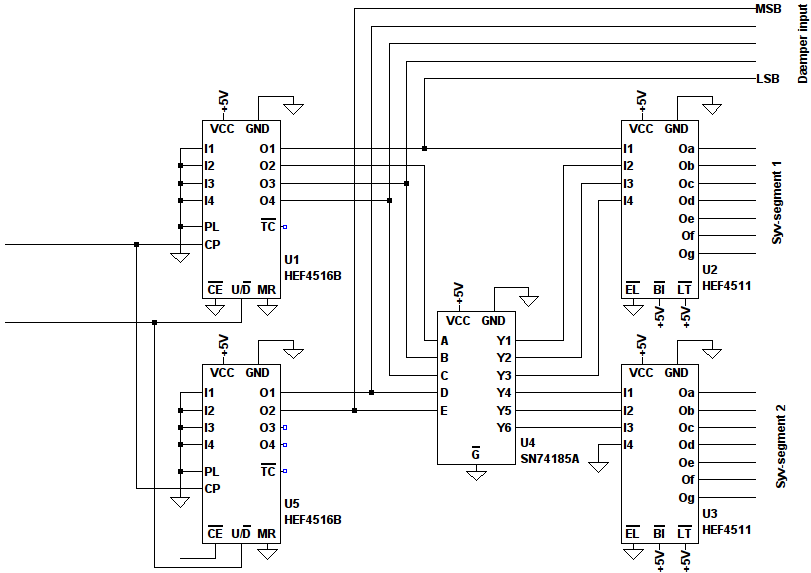
\includegraphics[width=\textwidth]{teknisk/volumenkontrol/taeller.png}
\caption{Diagram over tælleren og displaydriveren}
\label{fig:taeller}
\end{figure}

Tællerens opgave er at holde styr på hvad volumenniveauet er og diagrammet for den er vist på figur \ref{fig:taeller}. Der tælles op eller ned når der trykkes på én af de to volumenknapper. Hvor hurtigt der skal tælles, bestemmes af det AND'ede signal fra VCO'en og XOR-gaten. VCO'en fungerer som en clock på AND-gaten, mens XOR-signalet sørger for, at det kun er den ene knap der holdes nede. Hvis begge knapper holdes nede, vil XOR-signalet være lavt, og der vil intet signal blive sendt til tælleren. Om der skal tælles op eller ned, styres af et signal fra den knap der repræsenterer et ønske om en sænkning i volumeniveau. Hvis denne er nede, som den eneste knap, vil tælleren tælle ned af. Hvis denne ikke er nede, men XOR-signalet stadig er højt, betyder det at den anden knap er nede og tælleren vil derfor tælle op. Tælleren giver et binært output, som danner grundlag for hvad der vises i displayet og hvordan reguleringen af volumen indstilles. Tælleren der benyttes er en 4-bit tæller af typen HEF4516B \cite{hef4516b-datablad}. Da fire bit ikke er nok skal der bruges to tællere.
\fixme{Beregninger be here... or there}

Yderligere skal der også bruges kontrollogik, for at sikre tælleren ikke tæller for højt eller lavt og for at styre den anden tæller. Til at lave et endestop i den laveste ende af tællerens område, lægges alle tællerens output bits sammen i en OR-gate. Dette resultere i et nul, hvis tælleren står på nul. Der skal dog være mulighed for at tælle opad, når tælleren står på nul. Derfor skal UP/$\overline{\mathrm{DN}}$ signalet også med i OR-gaten, udgangssignalet vil nu være lavt når tælleren ikke må tælle nedad. Til at lave endestop i den høje ende, tages der udgangspunkt i en tæller værdi på 50, $110010_\mathrm{b}$. Da dette vil være maks værdien for tælleren er det kun de  udgange der er høje, der er af betydning. Når disse og UP/$\overline{\mathrm{DN}}$ signalet bliver samlet i en NAND-gate vil resultatet kun være lavt når der ikke må tælles højere. Dette signal AND'es sammen med signalet for det lave endstop og CLK signalet, dette bevirker at der ikke kommer CLK signal til de to tællere hvis de har ramt et af endestoppene.

Displaydriveren konverterer signalet fra tælleren til et signal der kan vises på de to 7-segment displays. Der konverteres fra tællerens binære output til BCD, Binary-coded decimal, for så at konvertere det til et signal 7-segment displaysne kan vise. Der benyttes en SN74185A \cite{sn74185a-datablad} til konverteringen fra binær til BCD. Fordelen ved at konvertere til BCD først er at denne konvertering også deler det binære tal op i to, en'ere og ti'ere. Disse to binære tal sendes igennem en 7-segmentsdriver, HEF4511 \cite{hef4511-datablad}, for at få et output der fungerer med 7-segmenterne. Displaydriveren er også vist på figur \ref{fig:taeller}.

\subsection*{Display}
\label{volumenkontrol-design-display}
Indstillingen af volumenkontrollen vises på to 7-segmenter. Dette er valgt, fordi disse er enkle at styre med simple kredsløb og det derfor ikke er nødvendigt med en microcontroller for at styre dem, som tilfældet havde været, hvis et LCD-display i stedet var blevet benyttet.

\subsection*{Dæmper}
\label{volumenkontrol-design-daemper}
Dæmperen er en en analog attenuator, som er sammensat af to sæt modstandsattenuatore, hver efterfulgt af en buffer. Dæmpningen indstilles ved at ændre, hvor signalet tages ud af de to modstandsattenuatore, ved brug af en analog multiplekser. Den første attenuator består af syv modstande, hvor der er en dæmpning på 8 dB mellem hver modstand. Den anden attenuatorer består af otte modstande, hvor der er en dæmpning på 1 dB mellem hver modstand. Det er således muligt at kombinere de to attenuatorer til at dæmpe signalet mellem 0 og 55 dB, med et interval på 1 dB. Diagrammet er afbilledet på figur \ref{fig:volumenkontrol_daemper} og modstandene derpå er beregnet i Appendiks C??.

\begin{figure}[h]
\centering
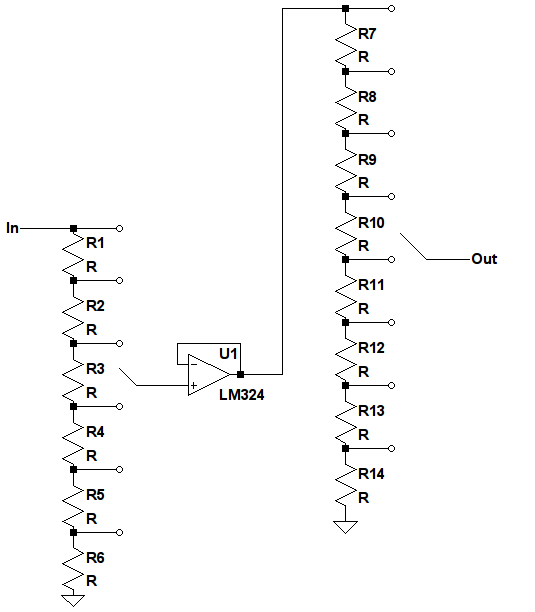
\includegraphics[width=\textwidth]{teknisk/volumenkontrol/daemper.png}
\caption{Diagram over dæmperen}
\label{fig:volumenkontrol_daemper}
\end{figure}

\clearpage
\section{Simulering}
\label{volumenkontrol-simulering}

På figur \ref{fig:volumenkontrol-diagram} er vist diagrammet, med komponent værdier, over volumenkontrollen til og med signalet til tælleren.

\begin{figure}[h]
\centering
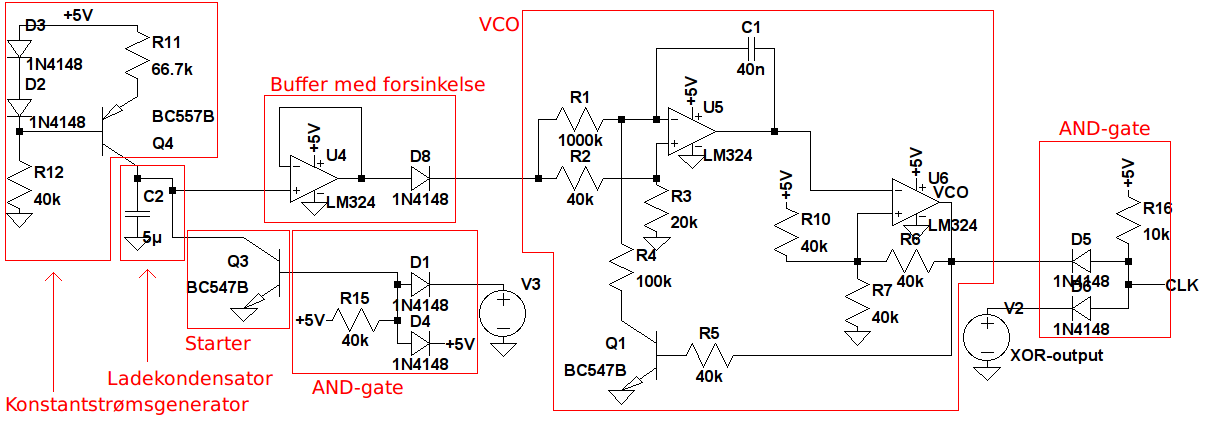
\includegraphics[width=\textwidth]{teknisk/volumenkontrol/diagram.png}
\caption{Diagram over volumenkontrollen}
\label{fig:volumenkontrol-diagram}
\end{figure}

På figur \ref{fig:vco-signal} ses resultatet af at påtrykke en konstant spænding på VCO'en. Dette resulterer i udgangen på integratoren, den blå kurve, svinger mellem schmitt-triggerens to niveauer med en fastdefineret frekvens. Det kan ses at plusindgangen på schmitt-triggeren, den røde kurve, er høj når integratorens udgang er opadgående og lav når den er nedadgående. 

\begin{figure}[h]
\centering
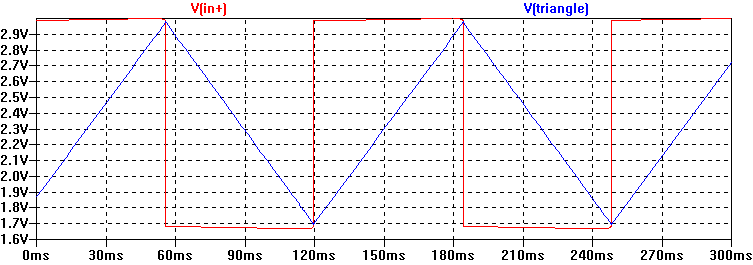
\includegraphics[width=\textwidth]{teknisk/volumenkontrol/vco-signal.png}
\caption{Integratorens udgang og plusindgangen på schmitt-triggeren}
\label{fig:vco-signal}
\end{figure}

Figur \ref{fig:stresstest} viser hvordan volumenkontrollen fungerer, når man trykker på en knap. Den blå graf, V(knap), viser knappens tilstand; når den er lav, er knappen trykket ned. Den lyseblå, V(clk) viser outputtet til clocken. Clocken på tælleren er flankestyret, hvilket vil sige, at der kun vil blive flyttet et trin, hver gang den lyseblå, V(clk) går fra lav til høj. Når knappen holdes nede, kan man se at kontrolspændingen, V(vc), stiger. Dette vil få spændingen på udgangen af integratoren, V(triangle), til at stige, indtil den rammer den høje trigger-spænding. Herefter vil spændingen falde igen, og oscillere hurtigere og hurtigere, i takt med at kontrolspændingen stiger. Ca. 3 sekunder efter at knappen trykkes ned, rammer kontrolspændingen sit max, som udregnet. Her vil udgangen på integratoren, og derfor også schmitt-triggeren, svinge med en frekvens på ca. 10 Hz.

\begin{figure}[h]
\centering
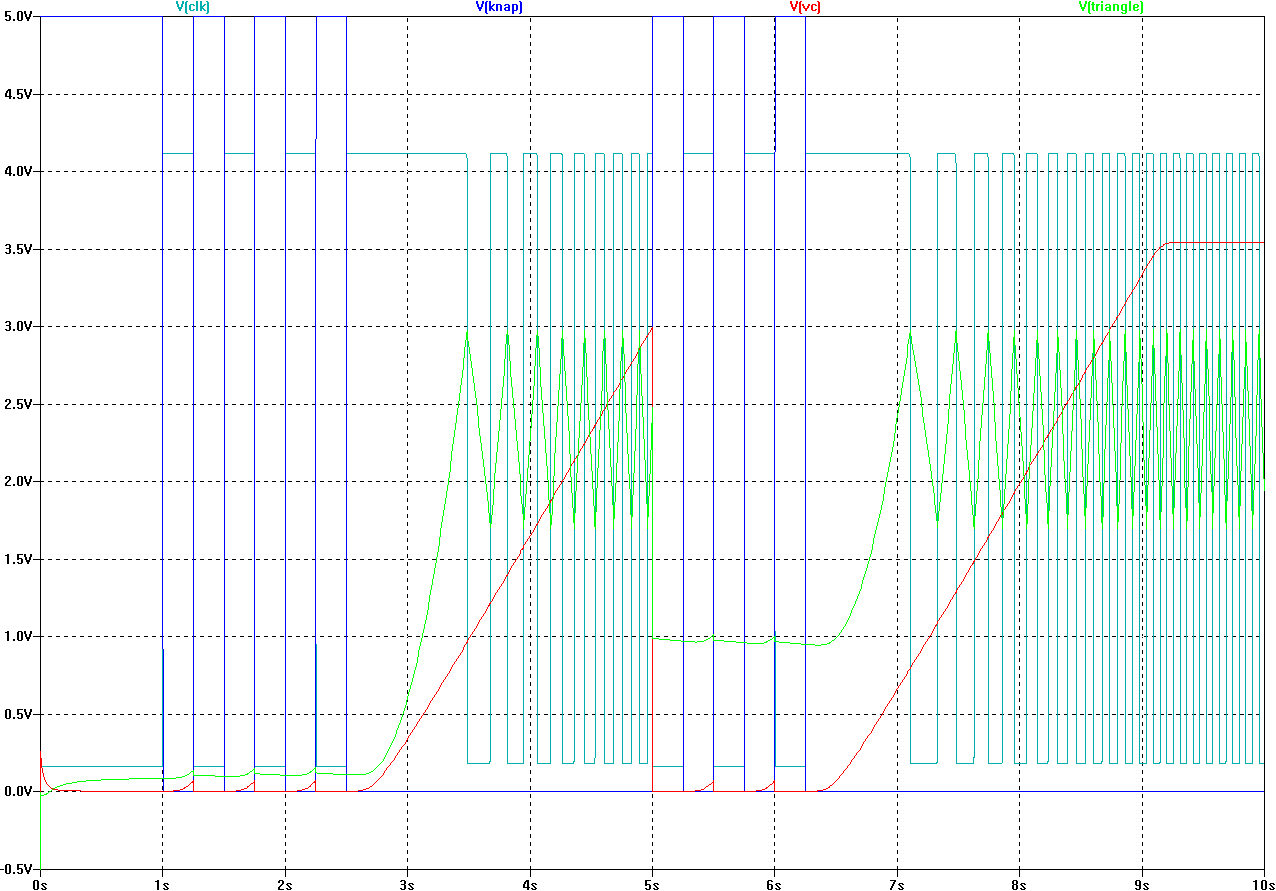
\includegraphics[width=\textwidth]{teknisk/volumenkontrol/stress-test.png}
\caption{Simulering af at trykke på og holde en knap nede.}
\label{fig:stresstest}
\end{figure}

På figur \ref{fig:konstantstroem} ses en simulering af konstantstrøms generatoren. Det er tydeligt at se, at konstantstrømsgeneratoren genererer en konstant strøm, Ic(Q4), indtil den ikke har et sted at løbe hen. Dette sker når kondensatoren er ladet op. Det er desuden tydeligt at se at kondensatoren, V(c2), bliver opladet lineært, med det samme knappen, V(knap), bliver trykket ned. 

\begin{figure}[h]
\centering
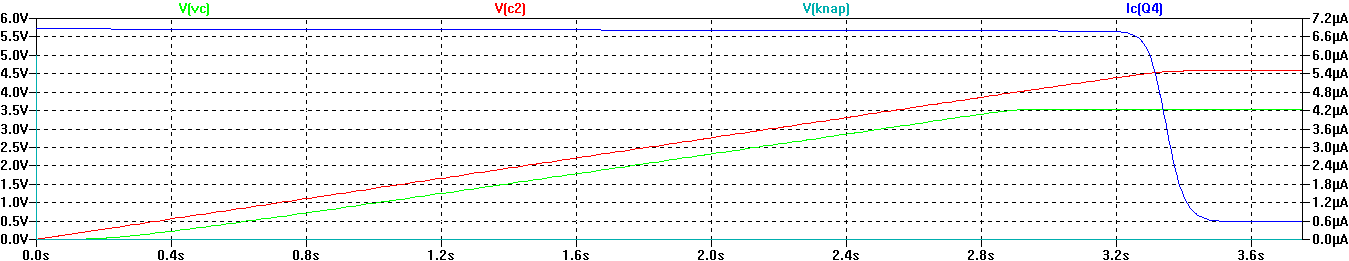
\includegraphics[width=\textwidth]{teknisk/volumenkontrol/konstantstroem.png}
\caption{Simulering af konstanstrømsgeneratoren}
\label{fig:konstantstroem}
\end{figure}

%Implementering
\chapter{Implementering}
\label{implementering}


%Accepttest
\chapter{Samlet accepttest}
\label{acceptest}
Efter systemet implementeredes, blev der udført målinger, som vist i appendiks \ref{maaling_hifi}. Ud fra disse kan der konkluderes at systemet lever op til størstedelen af de opstillede krav. 

\begin{table}[h]
\centering
\begin{tabular}{l|r|l|r}
\hline\hline
Område & Krav & Betingelse(r) & Status \\
\hline\hline
\multicolumn{4}{c}{\textbf{Teknisk:}} \\\hline
Forstærkerklasse & AB & & \checkmark\\[4pt]
Total Harmonic & < 1 \% & & $\mathcal{X}$ \\
Distortion & & $\circ$ < 0,5 \% i forforstærker & \checkmark\\
& & $\circ$ < 0,5 \% i effektforstærker & $\mathcal{X}$\\
& & $\circ$ Begge i effektområde & \\
& & ~~~fra 0 til -26 dB & \\[4pt]
Frekvensgang & 20 Hz - 20 kHz & $\circ$ $\pm$ 1,5 dB ved ref. 1 kHz & \checkmark\\
& & $\circ$ < 3 dB dæmpning & \\
& & ~~~fra 20 Hz til 63 Hz og  & \\
& & ~~~fra 12,5 kHz til 20 kHz & \\[4pt]
Indgangstyper & Linie og mikrofon & $\circ$ Med $"$Monacor & \checkmark \\
& & ~~~MCE-4000$"$ mikrofon & \\[4pt]
Antal trin i & 4 & & \checkmark\\
indgangsvælger & & & \\[4pt]
Dæmpning af slukket & > 50 dB & $\circ$ Ved 20 Hz - 20 kHz & \\
indgangssignal & & & \\[4pt]
Indgangsimpedans i & > 22 k\ohm & & \checkmark \\
liniesignalsindgang & & &\\[4pt]
Indgangsimpedans i & > 5 k\ohm & & \checkmark \\
mikrofonsignalsindgang & & & \\[4pt]
Equalizer-bånd & 3 & & $\mathcal{X}$ \\[4pt]
Styring af volumen- & Digital & & $\mathcal{X}$\\
kontrol & & &\\[4pt]
Dæmpningsområde i & 0 dB - 50 dB & $\circ$ 1 dB per niveau & \checkmark \\
volumenkontrol & & & \\[4pt]
Udgangseffekt & > 20 W & $\circ$ I 8~\ohm-højtaler & $\mathcal{X}$ \\[4pt]
Udgangssignaltype & Mono & & \checkmark \\[4pt]
Kortslutningsstrøm & 3 A & $\circ$ Som peakstrøm & $\mathcal{X}$ \\
i udgangen & & & \\\hline
\multicolumn{4}{c}{\textbf{Frontpanel (input):}} \\\hline
Indgangsvælger & Èn trykknap & & \checkmark\\[4pt]
Volumenkontrol & To trykknapper & & \checkmark \\[4pt]
Equalizer & Èn drejeknap pr. bånd & & $\mathcal{X}$ \\\hline
\multicolumn{4}{c}{\textbf{Frontpanel (output):}} \\\hline
Indgangsvælger & To lysdioder & $\circ$ Én per indgang & \checkmark\\[4pt]
Volumedisplay & To 7-segmenter & & \checkmark \\[4pt]
Visualizer & 6 lysdioder & $\circ$ 2 grønne, 2 gule, 2 røde & $\mathcal{X}$ \\
\hline\hline
\end{tabular}
\caption{Status af krav for hele systemet}
\label{tab:kravspec:accept}
\end{table}

%Konklusion
\chapter{Konklusion}
\label{konklusion}

Formålet med dette projekt var at designe en HiFi-forstærker med digital styring. Målet var at designe en forstærker med to indgange, mikrofon og liniesignal, forforstærker, indgangsvælger, volumenkontrol, equalizer, visualizer og effektforstærker. Disse moduler skulle leve op til kravspecifikationen, som består af gængse standarder og krav bestemt af projektgruppen. 
Alle moduler undtagen tonekontrollen blev designet og simuleret. Equalizer og visualizer blev udeladt på grund af tidsmangel. Kortslutningssikringen er det eneste modul som ikke blev bygget og testet grundet at det indledende design var fejlbehæftet og tidsmangel. De resterende moduler er bygget og testet, samt blevet vurderet med udgangspunkt i de opsatte krav. 
Forforstærkeren og indgangsvælgeren bestod alle de opstillede krav. Volumenkontrollen var fejlbehæftet da tælleren ikke var konsistent i op og nedtælling samt at den har 52 trin, hvor kravet var 51. 
Effektforstærkeren overholdt alle kravene bortset fra at den dæmpede for meget indenfor frekvensområdet 20 Hz - 20 kHz. 

Efter at alle moduler var blevet testet hver for sig blev HiFi-forstærkeren implementeret og testet. Testene på det samlede system viste at ingen af de opsatte krav blev overholdt. 

\bibliographystyle{plain}
\bibliography{referencer/referencer}

\listoffixmes

\end{document}